\subsection{服务端UI设计}
大致设计如下图所示, 页面中分为了多个模块,以医生个人信息模块为例,点击后即可展示医生个人信息。

\begin{figure}[htbp]
	\centering
	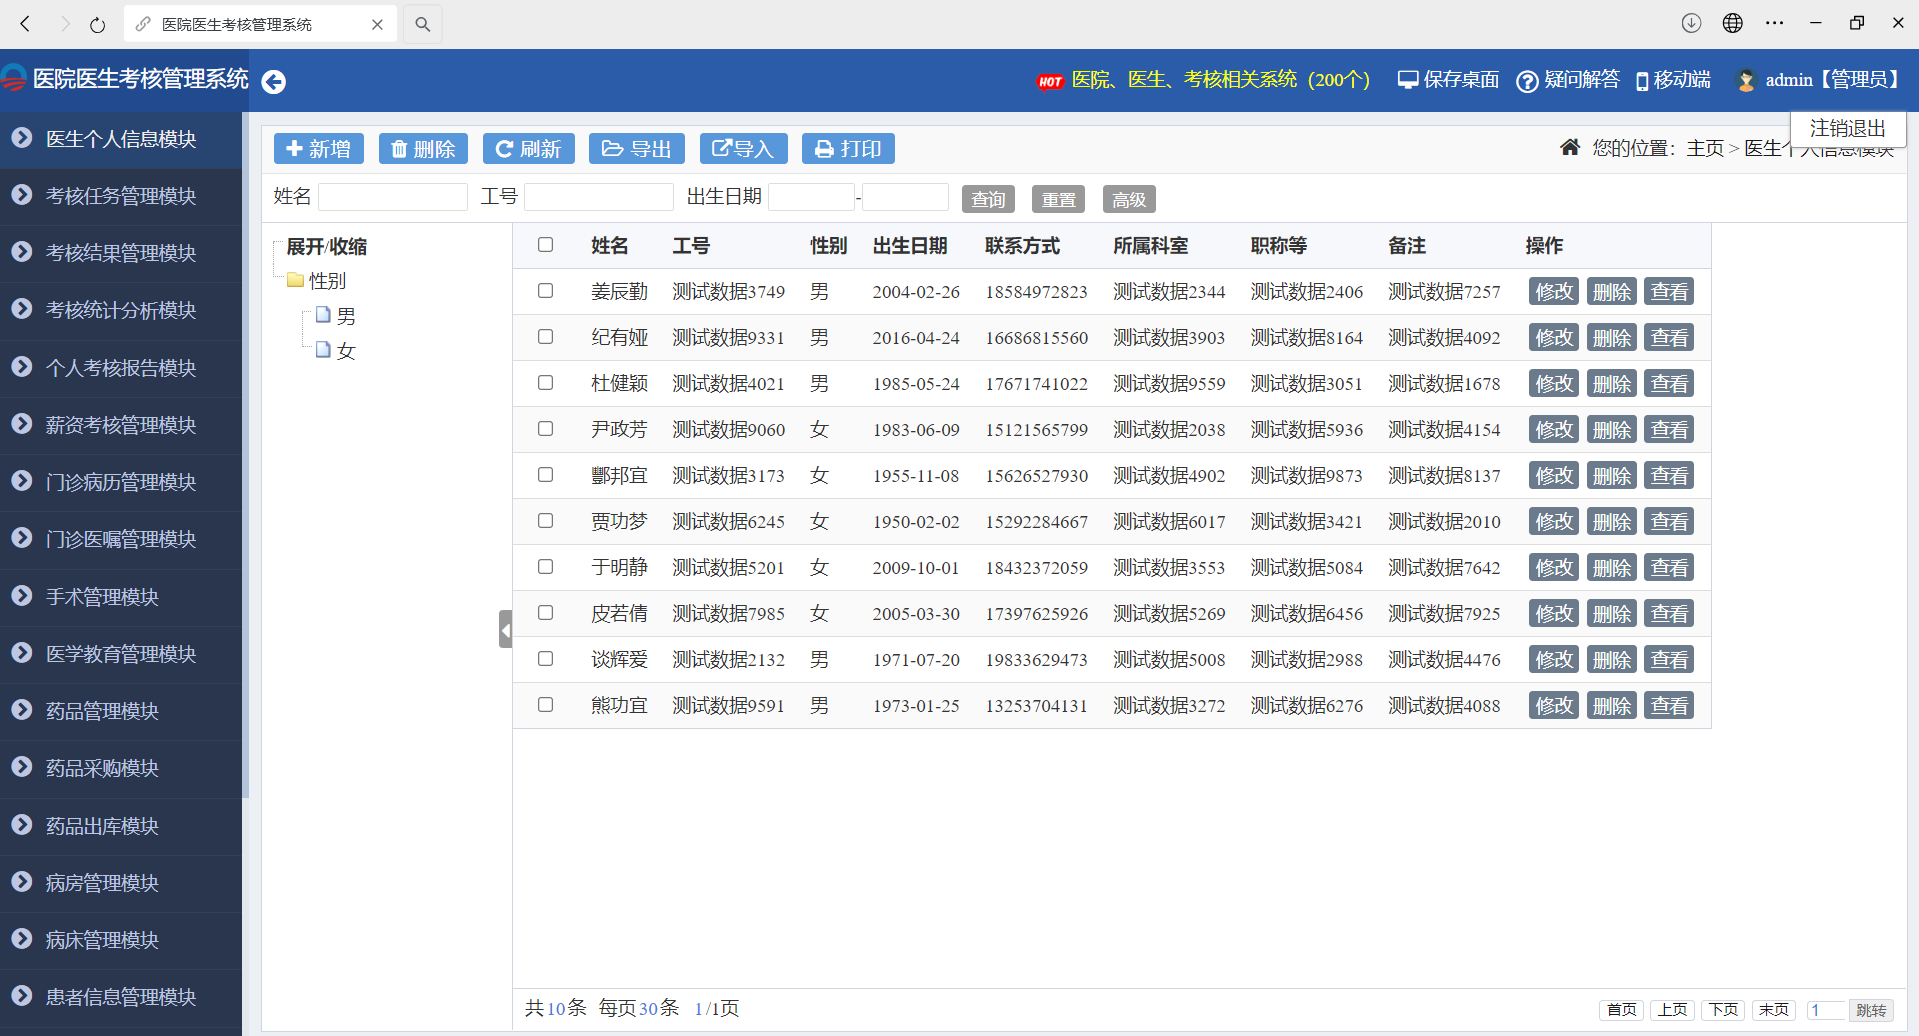
\includegraphics[width=0.9\textwidth]{figures/111.png}
	\caption{服务端UI设计}
\end{figure}

进一步点击可以查看和修改数据,并且支持数据的导出:


\begin{figure}[htbp]
	\centering
	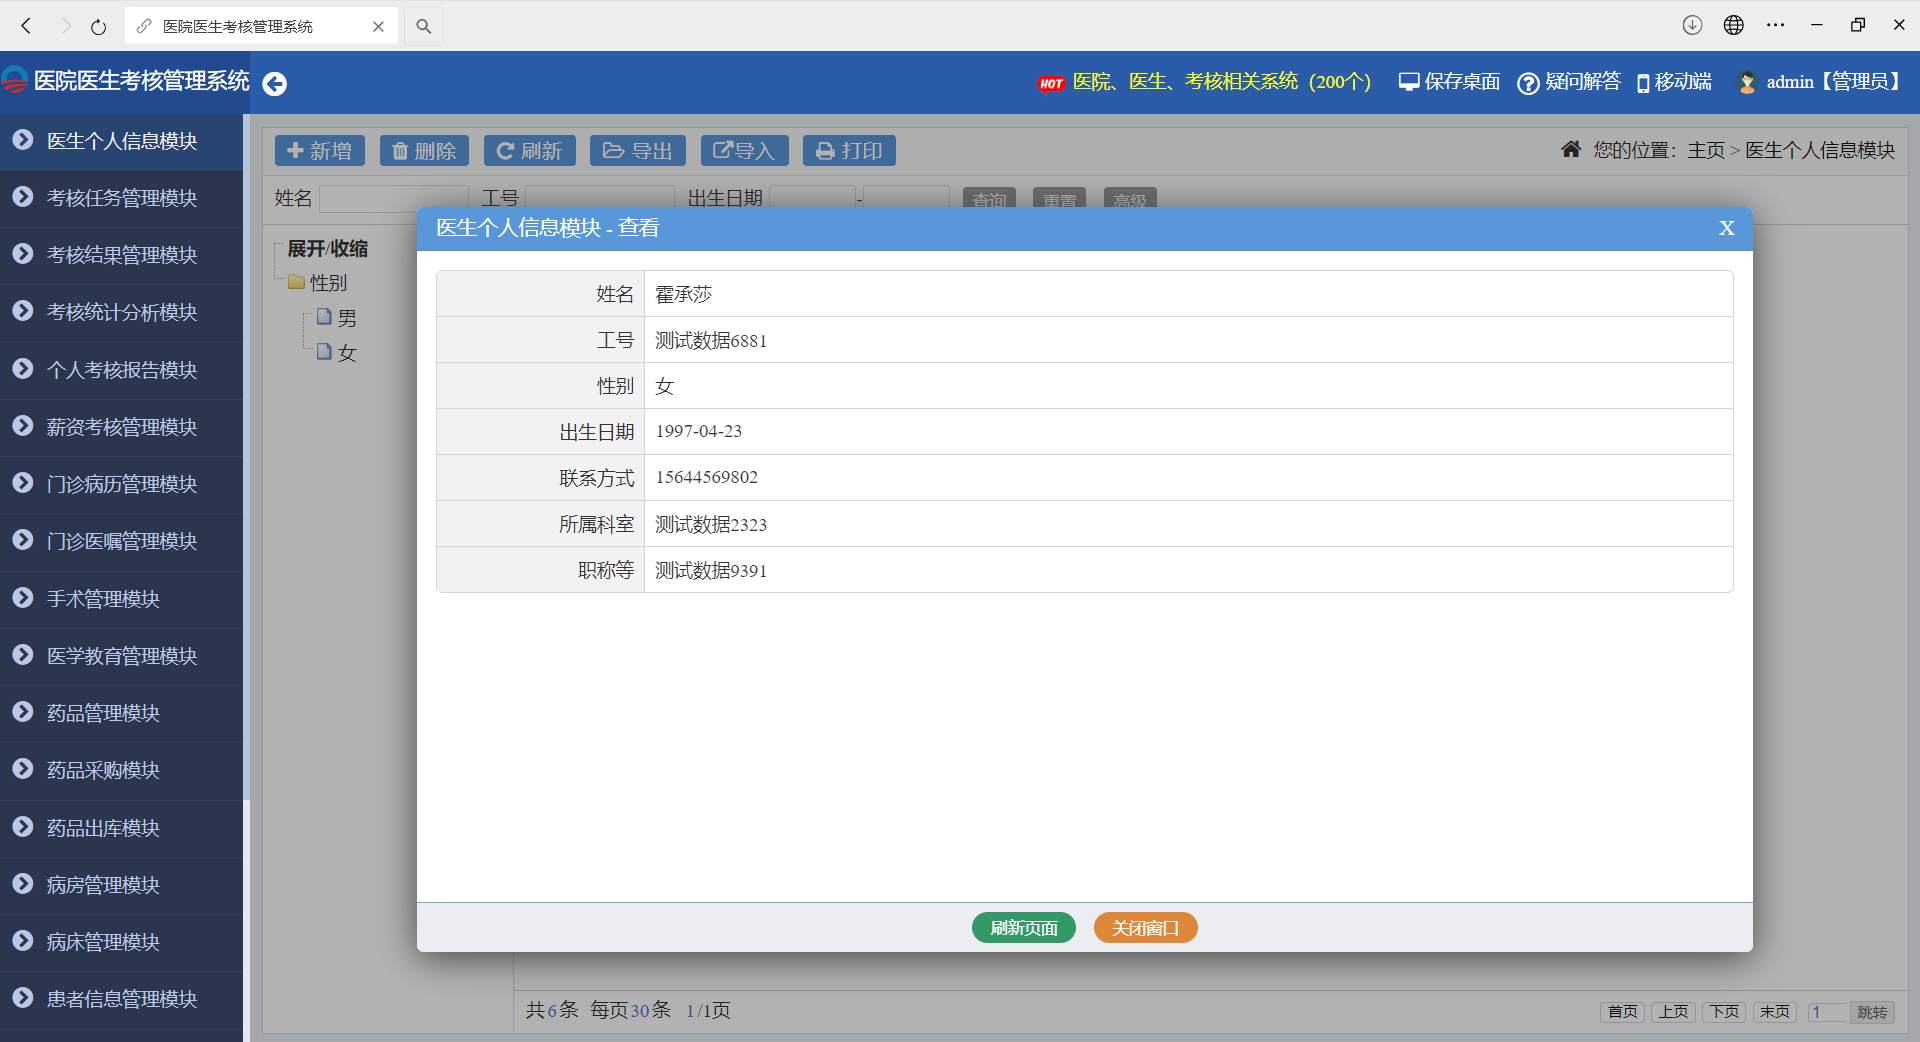
\includegraphics[width=0.9\textwidth]{figures/112.png}
	\caption{查看和修改数据页面展示}
\end{figure}

其余功能不在一一给出,所有设计的功能见下章节

\subsection{服务功能设计}
\subsubsection{用户注册与登录机制}

病人可以通过注册账户并登录系统,以便安全、便捷地使用系统提供的各项服务。

\begin{table}[htbp]
	\centering
	\begin{tabular}{|p{6cm}|p{6cm}|}
		\hline
		\textbf{注册} & \textbf{登录} \\
		\hline
		用户访问注册页面,填写必要信息(如用户名、密码、邮箱等),提交注册请求。 & 用户访问登录页面,输入注册时的用户名和密码。 \\
		系统验证用户提供的信息是否符合要求,若符合则完成注册,向用户发送确认邮件。 & 系统验证用户输入的用户名和密码是否匹配注册时记录的信息。 \\
		用户收到确认邮件,点击确认链接完成账户激活。 & 登录成功后,用户可以访问系统提供的各项服务。 \\
		\hline
	\end{tabular}
	\caption{用户注册与登录机制}
\end{table}

\begin{figure}[htbp]
	\centering
	\begin{tikzpicture}[node distance=1.5cm, >=stealth]
		
		% Define styles
		\tikzstyle{process} = [rectangle, minimum width=2.5cm, minimum height=0.5cm, text centered, draw=black, fill=orange!30, font=\footnotesize]
		\tikzstyle{decision} = [diamond, minimum width=2.5cm, minimum height=0.5cm, text centered, draw=black, fill=green!30, font=\footnotesize]
		
		% Define nodes
		\node (A) [process] {用户访问注册页面};
		\node (B) [process, below of=A] {填写必要信息};
		\node (C) [process, below of=B] {提交注册请求};
		\node (D) [decision, below of=C, yshift=-1.5cm] {验证是否符合要求};
		\node (E) [process, right of=D, xshift=3cm] {完成注册};
		\node (F) [process, below of=E] {发送确认邮件};
		\node (G) [process, below of=F] {用户点击确认链接};
		\node (H) [process, below of=G] {完成账户激活};
		\node (I) [process, below of=H] {用户可以登录系统};
		\node (J) [process, below of=I] {访问系统服务};
		
		% Define arrows
		\draw [->] (A) -- (B);
		\draw [->] (B) -- (C);
		\draw [->] (C) -- (D);
		\draw [->] (D) -- node[anchor=south] {符合} (E);
		\draw [->] (D) -- node[anchor=west] {不符合} (C);
		\draw [->] (E) -- (F);
		\draw [->] (F) -- (G);
		\draw [->] (G) -- (H);
		\draw [->] (H) -- (I);
		\draw [->] (I) -- (J);
		
	\end{tikzpicture}
	\caption{用户注册流程}
	\label{fig:registration}
\end{figure}

%\begin{figure}[h]
%	\centering
%	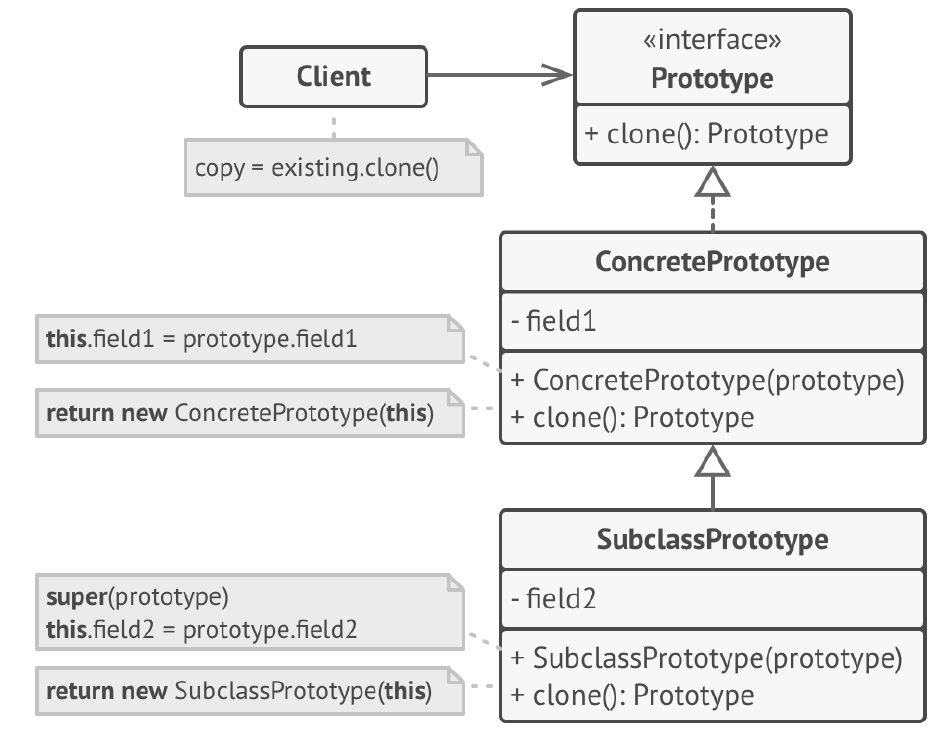
\includegraphics[width=0.4\textwidth]{figures/04.png} 
%	\caption{UML图}
%\end{figure}
\newpage
\subsubsection{个人医疗信息管理}
用户可以轻松查看、管理和更新自己的个人医疗信息,包括过往病史、药物过敏信息等,以确保信息的准确性和时效性。但是首先需要登录。

\begin{table}[htbp]
	\centering
	\begin{tabular}{|p{6cm}|p{6cm}|}
		\hline
		\textbf{操作} & \textbf{描述} \\
		\hline
		查看个人医疗信息 & 用户登录后,可以查看个人医疗信息,包括病史、药物过敏信息等。 \\
		更新个人医疗信息 & 用户可以更新病史、药物过敏等信息。需要通过系统审核确保信息的准确性。 \\
		授权访问 & 用户可以授权医生或家属访问特定的医疗信息。 \\
		查看访问记录 & 用户可以查看谁访问了他们的医疗记录,确保信息的安全。 \\
		接收系统提示 & 用户根据更新的医疗信息接收健康提示或提醒,比如药物相互作用警告。 \\
		\hline
	\end{tabular}
	\caption{个人医疗信息管理操作(更新版)}
\end{table}


\begin{figure}[htbp]
	\centering
	\begin{tikzpicture}[node distance=2.5cm, >=stealth, auto]
		
		% Define styles
		\tikzstyle{process} = [rectangle, minimum width=3cm, minimum height=1cm, text centered, draw=black, fill=blue!30, font=\footnotesize]
		\tikzstyle{decision} = [diamond, minimum width=3cm, minimum height=1cm, text centered, draw=black, fill=orange!30, font=\footnotesize]
		\tikzstyle{startstop} = [ellipse, minimum width=3cm, minimum height=1cm, text centered, draw=black, fill=red!30, font=\footnotesize]
		\tikzstyle{io} = [trapezium, trapezium left angle=70, trapezium right angle=-70, minimum width=3cm, minimum height=1cm, text centered, draw=black, fill=yellow!30, font=\footnotesize]
		
		% Define nodes
		\node (start) [startstop] {开始};
		\node (login) [process, below of=start] {用户登录系统};
		\node (navigate) [process, below of=login] {导航至个人信息页面};
		\node (chooseAction) [decision, below of=navigate, yshift=-1cm] {选择操作};
		\node (updateInfo) [process, below left of=chooseAction, xshift=-3cm, yshift=-0.5cm] {更新医疗信息};
		\node (authorize) [process, below right of=chooseAction, xshift=3cm, yshift=-0.5cm] {授权访问};
		\node (submitUpdate) [process, below of=updateInfo] {提交更新};
		\node (review) [process, below of=submitUpdate] {审核更新};
		\node (accessLog) [process, below of=authorize] {查看访问记录};
		\node (receiveAlerts) [process, below of=review] {接收健康提示};
		\node (end) [startstop, below of=chooseAction, yshift=-6cm] {结束};
		
		% Define arrows
		\draw [->] (start) -- (login);
		\draw [->] (login) -- (navigate);
		\draw [->] (navigate) -- (chooseAction);
		\draw [->] (chooseAction) -| node[anchor=south] {更新信息} (updateInfo);
		\draw [->] (chooseAction) -| node[anchor=south] {授权/查看记录} (authorize);
		\draw [->] (updateInfo) -- (submitUpdate);
		\draw [->] (submitUpdate) -- (review);
		\draw [->] (review) -- (receiveAlerts);
		\draw [->] (authorize) -- (accessLog);
		\draw [->] (receiveAlerts) |- (end);
		\draw [->] (accessLog) |- (end);
		
	\end{tikzpicture}
	\caption{个人医疗信息管理流程(更新版)}
	\label{fig:medical_info_management_updated}
\end{figure}

\newpage

\subsubsection{人工智能病情咨询服务}
集成AI技术,用户可以咨询自己的病情,并获得初步的医疗建议,为进一步的诊断和治疗提供参考。

\begin{table}[htbp]
	\centering
	\begin{tabular}{|p{6cm}|p{6cm}|}
		\hline
		\textbf{操作} & \textbf{描述} \\
		\hline
		提交病情描述 & 用户通过系统输入自己的症状和相关信息,作为咨询的基础。 \\
		AI分析病情 & 系统利用人工智能技术分析用户提交的信息,识别可能的病情。 \\
		获取医疗建议 & 根据AI分析结果,系统提供初步的医疗建议。 \\
		用户反馈 & 用户可以对提供的建议进行反馈,包括确认建议的有效性或请求更多信息。 \\
		医生审核 & 若用户请求,或AI系统不确定,医生会对病情进行人工审核,并提供进一步的建议。 \\
		追踪与跟进 & 系统定期追踪用户病情的变化,必要时提醒用户进行复查或更新病情信息。 \\
		\hline
	\end{tabular}
	\caption{人工智能病情咨询服务操作}
\end{table}


\begin{figure}[htbp]
	\centering
	\begin{tikzpicture}[node distance=2cm, >=stealth]
		
		% Define styles
		\tikzstyle{process} = [rectangle, minimum width=3cm, minimum height=1cm, text centered, draw=black, fill=green!30, font=\footnotesize]
		\tikzstyle{decision} = [diamond, minimum width=3cm, minimum height=1cm, text centered, draw=black, fill=orange!30, font=\footnotesize]
		\tikzstyle{startstop} = [ellipse, minimum width=3cm, minimum height=1cm, text centered, draw=black, fill=yellow!30, font=\footnotesize]
		
		% Define nodes
		\node (start) [startstop] {开始};
		\node (input) [process, below of=start] {提交病情描述};
		\node (analysis) [process, below of=input] {AI分析病情};
		\node (advice) [process, below of=analysis] {获取医疗建议};
		\node (feedback) [process, right of=advice, xshift=5cm] {用户反馈};
		\node (doctorReview) [process, below of=feedback] {医生审核};
		\node (trackFollowUp) [process, below of=doctorReview] {追踪与跟进};
		\node (end) [startstop, below of=advice] {结束};
		
		\node (decision) [decision, below of=advice, yshift=-5.5cm] {是否需要反馈或审核?};
		
		% Define arrows
		\draw [->] (start) -- (input);
		\draw [->] (input) -- (analysis);
		\draw [->] (analysis) -- (advice);
		\draw [->] (advice) -- (decision);
		\draw [->] (decision) -- node[anchor=east] {是} (feedback);
		\draw [->] (feedback) -- (doctorReview);
		\draw [->] (doctorReview) -- (trackFollowUp);
		\draw [->] (decision) -- node[anchor=south] {否} (end);
		\draw [->] (trackFollowUp) -| (end);
		
	\end{tikzpicture}
	\caption{人工智能病情咨询服务流程}
	\label{fig:ai_medical_consultation_service_updated}
\end{figure}
\newpage

\subsubsection{科室与专业领域介绍}
系统提供详细的科室信息,包括各科室的专业领域、医生团队介绍等,帮助用户了解并选择合适的科室。
此表格旨在展示系统提供的科室信息及其内容:
\begin{table}[htbp]
	\centering
	\begin{tabular}{|p{6cm}|p{6cm}|}
		\hline
		\textbf{科室名称} & \textbf{提供的信息} \\
		\hline
		内科 & 内科团队介绍、专业领域(如心脏病学、消化内科等)、常见病例处理 \\
		外科 & 外科团队介绍、专业领域(如普外科、神经外科等)、手术类型和案例 \\
		儿科 & 儿科团队介绍、儿童常见疾病处理、预防接种和健康管理 \\
		妇产科 & 妇产科团队介绍、孕期管理、生育服务和妇女健康问题 \\
		\hline
	\end{tabular}
	\caption{科室与专业领域介绍}
\end{table}
接下来,我们设计一个流程图来描述用户如何利用系统了解科室信息,并做出选择:
\begin{figure}[htbp]
	\centering
	\begin{tikzpicture}[node distance=2.5cm, >=stealth, auto]
		
		% Define styles
		\tikzstyle{process} = [rectangle, minimum width=3cm, minimum height=1cm, text centered, draw=black, fill=cyan!30, font=\footnotesize]
		\tikzstyle{decision} = [diamond, minimum width=3cm, minimum height=1cm, text centered, draw=black, fill=magenta!30, font=\footnotesize]
		\tikzstyle{startstop} = [ellipse, minimum width=3cm, minimum height=1cm, text centered, draw=black, fill=orange!30, font=\footnotesize]
		
		% Define nodes
		\node (start) [startstop] {开始};
		\node (login) [process, below of=start] {用户登录系统};
		\node (navigateToDepartment) [process, below of=login] {导航至科室介绍页面};
		\node (viewDepartments) [process, below of=navigateToDepartment] {查看科室列表};
		\node (selectDepartment) [process, below of=viewDepartments] {选择感兴趣的科室};
		\node (viewInfo) [process, below of=selectDepartment] {查看科室详细信息};
		\node (makeDecision) [decision, below of=viewInfo, yshift=-1cm] {是否选择此科室?};
		\node (endChoice) [process, right of=makeDecision, xshift=3cm] {结束选择};
		\node (end) [startstop, below of=makeDecision, yshift=-1cm] {结束};
		
		% Define arrows
		\draw [->] (start) -- (login);
		\draw [->] (login) -- (navigateToDepartment);
		\draw [->] (navigateToDepartment) -- (viewDepartments);
		\draw [->] (viewDepartments) -- (selectDepartment);
		\draw [->] (selectDepartment) -- (viewInfo);
		\draw [->] (viewInfo) -- (makeDecision);
		\draw [->] (makeDecision) -- node[anchor=south] {是} (endChoice);
		\draw [->] (makeDecision) -- node[anchor=east] {否} (selectDepartment);
		\draw [->] (endChoice) |- (end);
		
	\end{tikzpicture}
	\caption{科室选择流程}
	\label{fig:department_selection_process}
\end{figure}

\newpage

\subsubsection{医生预约时段选择}
用户可以查看医生的可选时段,并根据自己的时间安排进行预约,提高就诊的灵活性和便利性。
此表格展示了医生预约时段选择的相关操作及描述:
\begin{table}[htbp]
	\centering
	\begin{tabular}{|p{6cm}|p{6cm}|}
		\hline
		\textbf{操作} & \textbf{描述} \\
		\hline
		查看医生列表 & 用户可以浏览所有可预约的医生列表,包括医生的专业领域、评分及用户评价。 \\
		查看医生时段 & 选择一位医生后,用户可以查看该医生的可预约时段。 \\
		选择预约时段 & 用户根据自己的时间安排选择一个合适的预约时段。 \\
		确认预约 & 用户填写个人信息(如联系方式)并确认预约。 \\
		接收确认 & 预约成功后,用户将接收到预约确认信息,包括就诊时间和地点。 \\
		取消预约 & 用户可以在规定时间内取消预约,并重新安排。 \\
		提交评价 & 完成就诊后,用户可以提交对医生的评价。 \\
		医生推荐 & 根据用户的预约历史和评价,系统推荐医生。 \\
		\hline
	\end{tabular}
	\caption{医生预约时段选择操作}
\end{table}

下面是描述用户如何进行医生预约时段选择的流程图:
\begin{figure}[htbp]
	\centering
	\begin{tikzpicture}[node distance=2cm, >=stealth, auto]
		
		% Define styles
		\tikzstyle{process} = [rectangle, minimum width=3cm, minimum height=1cm, text centered, draw=black, fill=cyan!30, font=\footnotesize]
		\tikzstyle{decision} = [diamond, shape aspect=2, minimum width=3cm, minimum height=1cm, text centered, draw=black, fill=magenta!30, font=\footnotesize]
		\tikzstyle{startstop} = [ellipse, minimum width=3cm, minimum height=1cm, text centered, draw=black, fill=orange!30, font=\footnotesize]
		
		% Define nodes
		\node (start) [startstop] {开始};
		\node (viewDoctors) [process, below of=start] {查看医生列表};
		\node (selectDoctor) [process, below of=viewDoctors] {选择医生};
		\node (viewTimeslots) [process, below of=selectDoctor] {查看可预约时段};
		\node (chooseTimeslot) [process, below of=viewTimeslots] {选择预约时段};
		\node (confirmAppointment) [process, below of=chooseTimeslot] {填写信息并确认预约};
		\node (decision1) [decision, below of=confirmAppointment, yshift=-0.5cm] {是否取消预约?};
		\node (cancelAppointment) [process, below of=decision1, yshift=-0.5cm] {取消预约};
		\node (receiveConfirmation) [process, right of=decision1, xshift=2cm] {接收预约确认};
		\node (submitReview) [process, below of=cancelAppointment] {提交评价};
		\node (recommendDoctors) [process, below of=submitReview] {医生推荐};
		\node (end) [startstop, below of=recommendDoctors] {结束};
		
		% Define arrows
		\draw [->] (start) -- (viewDoctors);
		\draw [->] (viewDoctors) -- (selectDoctor);
		\draw [->] (selectDoctor) -- (viewTimeslots);
		\draw [->] (viewTimeslots) -- (chooseTimeslot);
		\draw [->] (chooseTimeslot) -- (confirmAppointment);
		\draw [->] (confirmAppointment) -- (decision1);
		\draw [->] (decision1) -- node [near start] {是} (cancelAppointment);
		\draw [->] (decision1) -- node [near start] {否} (receiveConfirmation);
		\draw [->] (cancelAppointment) -- (submitReview);
		\draw [->] (receiveConfirmation) |- (submitReview);
		\draw [->] (submitReview) -- (recommendDoctors);
		\draw [->] (recommendDoctors) -- (end);
		
	\end{tikzpicture}
	\caption{医生预约时段选择流程}
	\label{fig:doctor_appointment_selection_process}
\end{figure}
\newpage

\newpage

\subsubsection{医生选择与预约确认}
在选定时段后,用户可以根据自己的需求和医生的专业背景选择心仪的医生,并确认预约。
此表格将展示用户在选择医生和确认预约时需执行的操作和相应的描述:
\subsubsection{医生选择与预约确认}
在选定时段后,用户可以根据自己的需求和医生的专业背景选择心仪的医生,并确认预约。
此表格将展示用户在选择医生和确认预约时需执行的操作和相应的描述:
\begin{table}[htbp]
	\centering
	\begin{tabular}{|p{6cm}|p{6cm}|}
		\hline
		\textbf{操作} & \textbf{描述} \\
		\hline
		查看医生资料 & 用户可以查看各医生的详细资料,包括专业背景、擅长领域、工作经验及用户评价。 \\
		在线咨询 & 用户可以在线咨询医生,以便更好地了解医生的专业能力和态度。 \\
		选择医生 & 根据医生的资料和用户自己的需求,选择最适合的医生。 \\
		选择时段 & 用户选择医生后,根据可用时段表选择最合适的预约时间。 \\
		填写预约信息 & 输入必要的预约信息,如个人健康状况简介等。 \\
		修改/取消预约 & 用户可以在规定时间内修改或取消预约。 \\
		确认预约 & 完成所有信息的填写后,提交预约请求。系统会发送预约确认通知给用户。 \\
		预约反馈 & 预约后,用户可提交对预约过程的反馈。 \\
		预约跟踪 & 用户可以跟踪预约状态,包括提醒通知和就诊前的准备事项。 \\
		\hline
	\end{tabular}
	\caption{医生选择与预约确认操作}
\end{table}

接下来的流程图将描述用户如何进行医生的选择和预约确认的整个过程:
\begin{figure}[htbp]
	\centering
	\begin{tikzpicture}[node distance=2cm, >=stealth, auto]
		
		% Define styles
		\tikzstyle{process} = [rectangle, minimum width=3cm, minimum height=1cm, text centered, draw=black, fill=cyan!30, font=\footnotesize]
		\tikzstyle{decision} = [diamond, shape aspect=2, minimum width=3cm, minimum height=1cm, text centered, draw=black, fill=magenta!30, font=\footnotesize]
		\tikzstyle{startstop} = [ellipse, minimum width=3cm, minimum height=1cm, text centered, draw=black, fill=orange!30, font=\footnotesize]
		
		% Define nodes
		\node (start) [startstop] {开始};
		\node (viewDoctorInfo) [process, below of=start] {查看医生资料};
		\node (onlineConsultation) [process, below of=viewDoctorInfo] {在线咨询};
		\node (selectDoctor) [process, below of=onlineConsultation] {选择医生};
		\node (chooseTimeslot) [process, below of=selectDoctor] {选择时段};
		\node (fillInfo) [process, below of=chooseTimeslot] {填写预约信息};
		\node (modifyCancel) [decision, below of=fillInfo, yshift=-0.5cm] {修改/取消预约?};
		\node (confirmAppointment) [process, right of=modifyCancel, xshift=2cm] {确认预约};
		\node (appointmentFeedback) [process, below of=modifyCancel, yshift=-0.5cm] {预约反馈};
		\node (appointmentTracking) [process, below of=appointmentFeedback] {预约跟踪};
		\node (end) [startstop, below of=appointmentTracking] {结束};
		
		% Define arrows
		\draw [->] (start) -- (viewDoctorInfo);
		\draw [->] (viewDoctorInfo) -- (onlineConsultation);
		\draw [->] (onlineConsultation) -- (selectDoctor);
		\draw [->] (selectDoctor) -- (chooseTimeslot);
		\draw [->] (chooseTimeslot) -- (fillInfo);
		\draw [->] (fillInfo) -- (modifyCancel);
		\draw [->] (modifyCancel) -- node [near start] {是} (appointmentFeedback);
		\draw [->] (modifyCancel) -- node [near start] {否} (confirmAppointment);
		\draw [->] (confirmAppointment) |- (appointmentFeedback);
		\draw [->] (appointmentFeedback) -- (appointmentTracking);
		\draw [->] (appointmentTracking) -- (end);
		
	\end{tikzpicture}
	\caption{医生选择与预约确认流程}
	\label{fig:doctor_selection_and_appointment_confirmation}
\end{figure}
\newpage

\newpage
\subsubsection{医疗费用账单管理}
用户可以在线提交和查看自己的医疗费用账单,包括详细的费用清单和总计,便于费用的核对和理解。
此表格旨在展示与医疗费用账单管理相关的操作及其描述:
\begin{table}[htbp]
	\centering
	\begin{tabular}{|p{6cm}|p{6cm}|}
		\hline
		\textbf{操作} & \textbf{描述} \\
		\hline
		提交医疗费用账单 & 用户可以在线提交自己的医疗费用账单,包括上传相关的医疗费用凭证。 \\
		查看费用账单 & 用户可以查看已提交的医疗费用账单及其详细的费用清单和总计。 \\
		费用账单审核 & 系统自动或人工审核提交的费用账单及凭证,确保费用的准确性。 \\
		费用账单异议 & 用户可以对账单中的某些费用项提出异议,要求重新审核或解释。 \\
		接收审核结果 & 用户接收到费用账单审核的最终结果,包括是否接受异议及调整后的费用总计。 \\
		在线支付费用 & 用户可以选择在线支付经审核后的医疗费用。 \\
		\hline
	\end{tabular}
	\caption{医疗费用账单管理操作}
\end{table}
以下流程图将描述一个复杂的医疗费用账单管理流程,包括账单的提交、审核、异议处理和支付等步骤.这个流程图涵盖了从用户提交医疗费用账单开始的全过程,包括账单的审核、对审核结果的异议处理,以及接收最终审核结果后的在线支付步骤。这个设计旨在提供一个全面的视角,展示医疗费用管理过程中可能涉及的各个环节,确保用户可以轻松地管理和理解自己的医疗费用。
\begin{figure}[htbp]
	\centering
	\begin{tikzpicture}[node distance=2cm, >=stealth, auto]
		
		% Define styles
		\tikzstyle{process} = [rectangle, minimum width=3cm, minimum height=1cm, text centered, draw=black, fill=blue!30, font=\footnotesize]
		\tikzstyle{decision} = [diamond, minimum width=3cm, minimum height=1cm, text centered, draw=black, fill=orange!30, font=\footnotesize]
		\tikzstyle{startstop} = [ellipse, minimum width=3cm, minimum height=1cm, text centered, draw=black, fill=red!30, font=\footnotesize]
		\tikzstyle{io} = [trapezium, trapezium left angle=70, trapezium right angle=-70, minimum width=3cm, minimum height=1cm, text centered, draw=black, fill=yellow!30, font=\footnotesize]
		
		% Define nodes
		\node (start) [startstop] {开始};
		\node (submitBill) [process, below of=start] {提交医疗费用账单};
		\node (reviewBill) [process, below of=submitBill] {费用账单审核};
		\node (decision1) [decision, below of=reviewBill, yshift=-1cm] {审核是否通过?};
		\node (queryBill) [process, left of=decision1, xshift=-3cm] {费用账单异议};
		\node (finalizeBill) [process, below of=decision1, yshift=-1cm] {接收审核结果};
		\node (payBill) [process, below of=finalizeBill] {在线支付费用};
		\node (end) [startstop, below of=payBill] {结束};
		
		% Define arrows
		\draw [->] (start) -- (submitBill);
		\draw [->] (submitBill) -- (reviewBill);
		\draw [->] (reviewBill) -- (decision1);
		\draw [->] (decision1) -- node[anchor=south] {否} (queryBill);
		\draw [->] (queryBill) |- (reviewBill);
		\draw [->] (decision1) -- node[anchor=east] {是} (finalizeBill);
		\draw [->] (finalizeBill) -- (payBill);
		\draw [->] (payBill) -- (end);
		
	\end{tikzpicture}
	\caption{医疗费用账单管理流程}
	\label{fig:medical_bill_management_process}
\end{figure}
\newpage

\subsubsection{缴费与退费流程}
系统支持在线缴费和退费功能,简化了费用处理流程,减少了用户在医院的等待时间。
此表格将介绍用户在系统中进行缴费和退费时需要执行的操作及其相应的描述:
\begin{table}[htbp]
	\centering
	\begin{tabular}{|p{6cm}|p{6cm}|}
		\hline
		\textbf{操作} & \textbf{描述} \\
		\hline
		查看待缴费用 & 用户可以查看自己的待缴费用清单及总计。 \\
		选择缴费方式 & 用户选择合适的在线支付方式进行缴费,如信用卡、支付宝、微信等。 \\
		缴费确认 & 完成支付后,系统将显示缴费成功确认信息。 \\
		查看退费政策 & 用户可以查阅具体的退费政策,了解可能的退费条件和流程。 \\
		申请退费 & 在符合退费条件的情况下,用户可以提交退费申请,附上必要的证明材料。 \\
		退费审核 & 系统自动或人工审核退费申请及证明材料。 \\
		退费处理 & 审核通过后,系统将按照用户选择的方式退回费用。 \\
		接收退费确认 & 用户接收到退费成功的确认信息。 \\
		\hline
	\end{tabular}
	\caption{缴费与退费流程操作}
\end{table}
以下复杂的流程图将展示缴费与退费过程中可能涉及的多个决策点和步骤.在这个流程中,用户首先查看待缴费用,然后选择支付方式进行缴费,并接收缴费确认。同时,用户也可以查看退费政策,如果需要,可以提交退费申请并经过审核后完成退费,最终接收退费确认。这个流程图详细地展示了用户在缴费与退费过程中可能遇到的各种情况,确保用户能够清楚地了解和执行每一步。

\begin{figure}[htbp]
	\centering
	\begin{tikzpicture}[node distance=2cm, >=stealth, auto]
		
		% Define styles
		\tikzstyle{process} = [rectangle, minimum width=3cm, minimum height=1cm, text centered, draw=black, fill=cyan!30, font=\footnotesize]
		\tikzstyle{decision} = [diamond, minimum width=3cm, minimum height=1cm, text centered, draw=black, fill=magenta!30, aspect=2, font=\footnotesize]
		\tikzstyle{startstop} = [ellipse, minimum width=3cm, minimum height=1cm, text centered, draw=black, fill=orange!30, font=\footnotesize]
		
		% Define nodes
		\node (start) [startstop] {开始};
		\node (viewFees) [process, below of=start] {查看待缴费用};
		\node (choosePayment) [process, below of=viewFees] {选择缴费方式};
		\node (confirmPayment) [process, below of=choosePayment] {缴费确认};
		\node (viewRefundPolicy) [process, right of=viewFees, xshift=4cm] {查看退费政策};
		\node (applyRefund) [process, below of=viewRefundPolicy] {申请退费};
		\node (reviewRefund) [process, below of=applyRefund] {退费审核};
		\node (processRefund) [process, below of=reviewRefund] {退费处理};
		\node (confirmRefund) [process, below of=processRefund] {接收退费确认};
		\node (end) [startstop, below of=confirmPayment, yshift=-6cm] {结束};
		
		% Define arrows
		\draw [->] (start) -- (viewFees);
		\draw [->] (viewFees) -- (choosePayment);
		\draw [->] (choosePayment) -- (confirmPayment);
		\draw [->] (viewFees) -| (viewRefundPolicy);
		\draw [->] (viewRefundPolicy) -- (applyRefund);
		\draw [->] (applyRefund) -- (reviewRefund);
		\draw [->] (reviewRefund) -- (processRefund);
		\draw [->] (processRefund) -- (confirmRefund);
		\draw [->] (confirmPayment) |- (end);
		\draw [->] (confirmRefund) -| (end);
		
	\end{tikzpicture}
	\caption{缴费与退费流程图}
	\label{fig:payment_and_refund_process}
\end{figure}
\newpage

\subsubsection{电子处方查询}
用户可以在线查询医生开具的处方信息,包括药物名称、用法用量等,便于用户理解和遵循医嘱。
此表格展示了用户在线查询电子处方时的相关操作及其描述:
\begin{table}[htbp]
	\centering
	\begin{tabular}{|p{6cm}|p{6cm}|}
		\hline
		\textbf{操作} & \textbf{描述} \\
		\hline
		登录系统 & 用户需要登录系统以访问自己的电子处方信息。 \\
		选择查询处方 & 用户可以选择查看最新的处方或历史处方记录。 \\
		查看处方详情 & 展示选定处方的详细信息,包括药物名称、用法用量、开具医生等。 \\
		下载处方 & 用户可以下载处方信息,以便线下购药或备份。 \\
		咨询医生 & 若对处方有疑问,用户可以通过系统向开具处方的医生发起咨询。 \\
		评价服务 & 完成处方查询和使用后,用户可以对服务进行评价。 \\
		\hline
	\end{tabular}
	\caption{电子处方查询操作}
\end{table}

下面的流程图将展示一个涵盖多个可能操作和选择的复杂电子处方查询流程。这个流程图从用户登录系统开始,之后用户可以选择查看最新或历史的处方记录,查看处方详情,并根据需要决定是否下载处方。如果对处方有疑问,用户还可以选择咨询医生。最后,用户可以对使用过程中的服务进行评价。此流程图考虑了用户在查询电子处方过程中可能的各种行为,使其成为一个全面且复杂的流程描述。
\begin{figure}[htbp]
	\centering
	\begin{tikzpicture}[node distance=2cm, >=stealth, auto]
		
		% Define styles
		\tikzstyle{process} = [rectangle, minimum width=3cm, minimum height=1cm, text centered, draw=black, fill=blue!30, font=\footnotesize]
		\tikzstyle{decision} = [diamond, minimum width=3cm, minimum height=1cm, text centered, draw=black, fill=orange!30, aspect=2, font=\footnotesize]
		\tikzstyle{startstop} = [ellipse, minimum width=3cm, minimum height=1cm, text centered, draw=black, fill=red!30, font=\footnotesize]
		\tikzstyle{io} = [trapezium, trapezium left angle=70, trapezium right angle=-70, minimum width=3cm, minimum height=1cm, text centered, draw=black, fill=yellow!30, font=\footnotesize]
		
		% Define nodes
		\node (start) [startstop] {开始};
		\node (login) [process, below of=start] {登录系统};
		\node (selectPrescription) [process, below of=login] {选择查询处方};
		\node (viewDetails) [process, below of=selectPrescription] {查看处方详情};
		\node (decision1) [decision, below of=viewDetails, yshift=-1.5cm] {是否下载处方?};
		\node (download) [process, left of=decision1, xshift=-3cm] {下载处方};
		\node (consult) [process, right of=decision1, xshift=3cm] {咨询医生};
		\node (review) [process, below of=decision1, yshift=-1.5cm] {评价服务};
		\node (end) [startstop, below of=review] {结束};
		
		% Define arrows
		\draw [->] (start) -- (login);
		\draw [->] (login) -- (selectPrescription);
		\draw [->] (selectPrescription) -- (viewDetails);
		\draw [->] (viewDetails) -- (decision1);
		\draw [->] (decision1) -- node[anchor=south] {是} (download);
		\draw [->] (decision1) -- node[anchor=south] {否} (consult);
		\draw [->] (download) |- (review);
		\draw [->] (consult) |- (review);
		\draw [->] (decision1) -- node[anchor=east] {不需要} (review);
		\draw [->] (review) -- (end);
		
	\end{tikzpicture}
	\caption{电子处方查询流程}
	\label{fig:electronic_prescription_query_process}
\end{figure}
\newpage


\subsubsection{电子病历搜索与访问}
用户可以搜索并查看自己的电子病历,包括历史就诊记录、检查结果等,便于健康管理和疾病预防。
此表格将介绍用户在线查看电子病历时的相关操作及其描述:
\begin{table}[htbp]
	\centering
	\begin{tabular}{|p{6cm}|p{6cm}|}
		\hline
		\textbf{操作} & \textbf{描述} \\
		\hline
		登录系统 & 用户需要登录系统以访问自己的电子病历信息。 \\
		搜索病历 & 用户可以根据日期、疾病名称或医生姓名等关键词搜索相关的电子病历。 \\
		选择病历记录 & 从搜索结果中选择特定的病历记录以查看详细信息。 \\
		查看病历详情 & 显示选定病历的详细信息,包括诊断、治疗过程、检查结果等。 \\
		下载病历 & 用户可以下载电子病历的副本,以便离线查看或备份。 \\
		咨询医生 & 若对病历内容有疑问,用户可以通过系统向相关医生发起咨询。 \\
		\hline
	\end{tabular}
	\caption{电子病历搜索与访问操作}
\end{table}

下面的流程图将展示一个包含多个分支和决策点的复杂电子病历搜索与访问流程。这个流程图从用户登录系统开始,接着用户可以搜索特定的电子病历记录,并选择查看病历详情。根据需要,用户可以决定是否下载病历的副本。如果对病历内容有疑问,还可以选择咨询相关的医生。此流程图包含了多个选择和操作,旨在详细描述电子病历搜索与访问的全过程。

\begin{figure}[htbp]
	\centering
	\begin{tikzpicture}[node distance=2cm, >=stealth, auto]
		
		% Define styles
		\tikzstyle{process} = [rectangle, minimum width=3cm, minimum height=1cm, text centered, draw=black, fill=cyan!30, font=\footnotesize]
		\tikzstyle{decision} = [diamond, minimum width=3cm, minimum height=1cm, text centered, draw=black, fill=magenta!30, aspect=2, font=\footnotesize]
		\tikzstyle{startstop} = [ellipse, minimum width=3cm, minimum height=1cm, text centered, draw=black, fill=orange!30, font=\footnotesize]
		\tikzstyle{io} = [trapezium, trapezium left angle=70, trapezium right angle=-70, minimum width=3cm, minimum height=1cm, text centered, draw=black, fill=yellow!30, font=\footnotesize]
		
		% Define nodes
		\node (start) [startstop] {开始};
		\node (login) [process, below of=start] {登录系统};
		\node (searchEMR) [process, below of=login] {搜索病历};
		\node (selectRecord) [process, below of=searchEMR] {选择病历记录};
		\node (viewDetails) [process, below of=selectRecord] {查看病历详情};
		\node (decision1) [decision, below of=viewDetails, yshift=-1.5cm] {需要下载病历?};
		\node (downloadEMR) [process, left of=decision1, xshift=-3cm] {下载病历};
		\node (consultDoctor) [process, right of=decision1, xshift=3cm] {咨询医生};
		\node (end) [startstop, below of=decision1, yshift=-1.5cm] {结束};
		
		% Define arrows
		\draw [->] (start) -- (login);
		\draw [->] (login) -- (searchEMR);
		\draw [->] (searchEMR) -- (selectRecord);
		\draw [->] (selectRecord) -- (viewDetails);
		\draw [->] (viewDetails) -- (decision1);
		\draw [->] (decision1) -- node[anchor=south] {是} (downloadEMR);
		\draw [->] (decision1) -- node[anchor=south] {否} (consultDoctor);
		\draw [->] (downloadEMR) |- (end);
		\draw [->] (consultDoctor) |- (end);
		
	\end{tikzpicture}
	\caption{电子病历搜索与访问流程}
	\label{fig:electronic_medical_record_search_and_access_process}
\end{figure}
\newpage

\subsubsection{预约挂号与问诊服务}
用户可以方便地预约挂号,并在预约时间进行在线或线下问诊,确保医疗服务的连续性和及时性。
此表格展示了用户预约挂号与问诊时的相关操作及其描述:
\begin{table}[htbp]
	\centering
	\begin{tabular}{|p{6cm}|p{6cm}|}
		\hline
		\textbf{操作} & \textbf{描述} \\
		\hline
		选择医生或科室 & 用户可以根据自己的需求选择特定的医生或科室进行预约。 \\
		确定预约时间 & 用户从可用的时间段中选择一个最适合自己的时间进行预约。 \\
		填写个人信息 & 用户需填写个人信息,如姓名、联系方式等,以完成预约挂号。 \\
		预约确认 & 系统确认用户的预约请求,并发送预约详情给用户。 \\
		进行问诊 & 在预约时间,用户可以选择在线问诊或到医院进行线下问诊。 \\
		问诊结束 & 问诊结束后,医生提供诊断结果和治疗建议。 \\
		\hline
	\end{tabular}
	\caption{预约挂号与问诊服务操作}
\end{table}
以下复杂的流程图展示了从预约挂号到完成问诊的整个过程,包括多个操作和决策点。在这个流程图中,用户首先选择合适的医生或科室,然后选择一个预约时间并填写个人信息以完成预约挂号。预约确认后,用户需要决定是进行在线问诊还是到医院进行线下问诊。问诊结束后,医生将提供诊断结果和治疗建议。这个设计考虑了预约挂号与问诊服务中可能的各种情况,确保了医疗服务的连续性和及时性。
\begin{figure}[htbp]
	\centering
	\begin{tikzpicture}[node distance=2cm, >=stealth, auto]
		
		% Define styles
		\tikzstyle{process} = [rectangle, minimum width=3cm, minimum height=1cm, text centered, draw=black, fill=cyan!30, font=\footnotesize]
		\tikzstyle{decision} = [diamond, minimum width=3cm, minimum height=1cm, text centered, draw=black, fill=magenta!30, aspect=2, font=\footnotesize]
		\tikzstyle{startstop} = [ellipse, minimum width=3cm, minimum height=1cm, text centered, draw=black, fill=orange!30, font=\footnotesize]
		
		% Define nodes
		\node (start) [startstop] {开始};
		\node (selectDoctor) [process, below of=start] {选择医生或科室};
		\node (chooseTime) [process, below of=selectDoctor] {确定预约时间};
		\node (fillInfo) [process, below of=chooseTime] {填写个人信息};
		\node (confirmAppointment) [process, below of=fillInfo] {预约确认};
		\node (decideMode) [decision, below of=confirmAppointment, yshift=-1.5cm] {问诊方式};
		\node (onlineConsultation) [process, left of=decideMode, xshift=-3cm] {在线问诊};
		\node (offlineConsultation) [process, right of=decideMode, xshift=3cm] {线下问诊};
		\node (consultationEnd) [process, below of=decideMode, yshift=-1.5cm] {问诊结束};
		\node (end) [startstop, below of=consultationEnd] {结束};
		
		% Define arrows
		\draw [->] (start) -- (selectDoctor);
		\draw [->] (selectDoctor) -- (chooseTime);
		\draw [->] (chooseTime) -- (fillInfo);
		\draw [->] (fillInfo) -- (confirmAppointment);
		\draw [->] (confirmAppointment) -- (decideMode);
		\draw [->] (decideMode) -- node[anchor=south] {在线} (onlineConsultation);
		\draw [->] (decideMode) -- node[anchor=south] {线下} (offlineConsultation);
		\draw [->] (onlineConsultation) |- (consultationEnd);
		\draw [->] (offlineConsultation) |- (consultationEnd);
		\draw [->] (decideMode) -- node[anchor=east] {决定} (consultationEnd);
		\draw [->] (consultationEnd) -- (end);
		
	\end{tikzpicture}
	\caption{预约挂号与问诊服务流程}
	\label{fig:appointment_registration_and_consultation_service_process}
\end{figure}
\newpage

\subsubsection{时段灵活性与个性化预约}
用户可以根据自己的时间安排,选择最佳的就诊时段,系统还会提供个性化的预约建议,以满足不同用户的需求。
此表格展示了与时段灵活性和个性化预约相关的操作及其描述:
\begin{table}[htbp]
	\centering
	\begin{tabular}{|p{6cm}|p{6cm}|}
		\hline
		\textbf{操作} & \textbf{描述} \\
		\hline
		登录系统 & 用户需要登录系统以访问预约功能。 \\
		输入个人偏好 & 用户可以输入自己的时间偏好、医生偏好等信息。 \\
		接收预约建议 & 系统根据用户输入的偏好提供个性化的预约建议。 \\
		选择紧急预约选项 & 如有紧急情况,用户可以选择紧急预约,享有优先预约权。 \\
		选择就诊时段 & 用户从系统提供的建议中选择最适合自己的就诊时段。 \\
		确认预约 & 用户确认预约详情并完成预约过程。 \\
		预约成功 & 系统发送预约成功的通知,包括就诊时间和地点等信息。 \\
		就诊后评价 & 用户就诊后,可以提交对医生和就诊体验的评价。 \\
		自动更新偏好 & 系统根据用户的历史预约信息和评价自动更新个人偏好。 \\
		\hline
	\end{tabular}
	\caption{时段灵活性与个性化预约操作}
\end{table}

面的流程图将展示从登录系统到完成预约的整个过程,包括多个操作和决策点。在这个流程图中,用户首先登录系统并输入个人偏好信息,如可用的时间段和偏好的医生类型等。系统根据用户的偏好提供个性化的预约建议。用户从中选择一个最适合自己的就诊时段并确认预约。最后,用户接收到预约成功的通知。这个设计旨在提供灵活的时段选择和个性化的预约建议,以满足不同用户的需求。
\begin{figure}[htbp]
	\centering
	\begin{tikzpicture}[node distance=2cm, >=stealth, auto]
		
		% Define styles
		\tikzstyle{process} = [rectangle, minimum width=3cm, minimum height=1cm, text centered, draw=black, fill=cyan!30, font=\footnotesize]
		\tikzstyle{decision} = [diamond, minimum width=3cm, minimum height=1cm, text centered, draw=black, fill=magenta!30, aspect=2, font=\footnotesize]
		\tikzstyle{startstop} = [ellipse, minimum width=3cm, minimum height=1cm, text centered, draw=black, fill=orange!30, font=\footnotesize]
		
		% Define nodes
		\node (start) [startstop] {开始};
		\node (login) [process, below of=start] {登录系统};
		\node (inputPreferences) [process, below of=login] {输入个人偏好};
		\node (receiveSuggestions) [process, below of=inputPreferences] {接收预约建议};
		\node (emergencyOption) [decision, right of=receiveSuggestions, xshift=2cm] {是否紧急预约?};
		\node (chooseTimeslot) [process, below of=receiveSuggestions] {选择就诊时段};
		\node (confirmAppointment) [process, below of=chooseTimeslot] {确认预约};
		\node (appointmentSuccess) [process, below of=confirmAppointment] {预约成功};
		\node (postAppointmentReview) [process, below of=appointmentSuccess] {就诊后评价};
		\node (updatePreferences) [process, below of=postAppointmentReview] {自动更新偏好};
		\node (end) [startstop, below of=updatePreferences] {结束};
		
		% Define arrows
		\draw [->] (start) -- (login);
		\draw [->] (login) -- (inputPreferences);
		\draw [->] (inputPreferences) -- (receiveSuggestions);
		\draw [->] (receiveSuggestions) -- (emergencyOption);
		\draw [->] (emergencyOption) -- node [near start] {是} (confirmAppointment);
		\draw [->] (emergencyOption) -- node [near start] {否} (chooseTimeslot);
		\draw [->] (receiveSuggestions) -- (chooseTimeslot);
		\draw [->] (chooseTimeslot) -- (confirmAppointment);
		\draw [->] (confirmAppointment) -- (appointmentSuccess);
		\draw [->] (appointmentSuccess) -- (postAppointmentReview);
		\draw [->] (postAppointmentReview) -- (updatePreferences);
		\draw [->] (updatePreferences) -- (end);
		
	\end{tikzpicture}
	\caption{时段灵活性与个性化预约流程}
	\label{fig:flexible_scheduling_and_personalized_appointment_process}
\end{figure}
\newpage
\subsubsection{电子问诊单与后续跟进}
问诊后,用户可以接收到电子问诊单,便于记录和后续跟进,确保医疗服务的完整性。
此表格展示了与电子问诊单接收和后续跟进相关的操作及其描述:
\begin{table}[htbp]
	\centering
	\begin{tabular}{|p{6cm}|p{6cm}|}
		\hline
		\textbf{操作} & \textbf{描述} \\
		\hline
		完成问诊 & 用户完成在线或线下问诊后,系统自动生成电子问诊单。 \\
		查看问诊单 & 用户可以在系统中查看电子问诊单的内容,包括诊断结果、治疗建议等。 \\
		下载问诊单 & 用户有选项下载问诊单,以便于打印或电子存档。 \\
		咨询医生 & 对问诊单有疑问的用户可以直接通过系统咨询医生。 \\
		安排后续治疗 & 根据问诊单的建议,用户可以安排后续的治疗或复诊。 \\
		\hline
	\end{tabular}
	\caption{电子问诊单与后续跟进操作}
\end{table}
下面的流程图将展示一个包含多个步骤和决策点的复杂电子问诊单接收与后续跟进流程。在这个流程图中,用户首先完成在线或线下问诊,随后系统将自动生成电子问诊单。用户可以查看问诊单的详细内容,包括医生的诊断结果和治疗建议。用户有选项下载问诊单,若对问诊单内容有疑问或需要进一步的指导,可以选择咨询医生。根据问诊单的建议,用户还可以安排后续的治疗计划或复诊。这个设计旨在确保医疗服务的完整性,同时提供了灵活的后续跟进选项。

\begin{figure}[htbp]
	\centering
	\begin{tikzpicture}[node distance=2cm, >=stealth, auto]
		
		% Define styles
		\tikzstyle{process} = [rectangle, minimum width=3cm, minimum height=1cm, text centered, draw=black, fill=cyan!30, font=\footnotesize]
		\tikzstyle{decision} = [diamond, minimum width=3cm, minimum height=1cm, text centered, draw=black, fill=magenta!30, aspect=2, font=\footnotesize]
		\tikzstyle{startstop} = [ellipse, minimum width=3cm, minimum height=1cm, text centered, draw=black, fill=orange!30, font=\footnotesize]
		
		% Define nodes
		\node (start) [startstop] {开始};
		\node (consultationEnd) [process, below of=start] {完成问诊};
		\node (viewConsultation) [process, below of=consultationEnd] {查看问诊单};
		\node (downloadDecision) [decision, below of=viewConsultation, yshift=-1.5cm] {是否下载问诊单?};
		\node (downloadConsultation) [process, left of=downloadDecision, xshift=-3cm] {下载问诊单};
		\node (consultDoctor) [process, right of=downloadDecision, xshift=3cm] {咨询医生};
		\node (arrangeTreatment) [process, below of=downloadDecision, yshift=-1.5cm] {安排后续治疗};
		\node (end) [startstop, below of=arrangeTreatment] {结束};
		
		% Define arrows
		\draw [->] (start) -- (consultationEnd);
		\draw [->] (consultationEnd) -- (viewConsultation);
		\draw [->] (viewConsultation) -- (downloadDecision);
		\draw [->] (downloadDecision) -- node[anchor=south] {是} (downloadConsultation);
		\draw [->] (downloadDecision) -- node[anchor=south] {否} (consultDoctor);
		\draw [->] (downloadDecision) -- node[anchor=east] {咨询结束} (arrangeTreatment);
		\draw [->] (downloadConsultation) |- (arrangeTreatment);
		\draw [->] (consultDoctor) |- (arrangeTreatment);
		\draw [->] (arrangeTreatment) -- (end);
		
	\end{tikzpicture}
	\caption{电子问诊单与后续跟进流程}
	\label{fig:electronic_consultation_form_and_follow_up_process}
\end{figure}

\newpage

\subsubsection{医疗服务评价体系参与}
用户可以参与对医生和医院服务的评价,为其他患者提供参考,同时也帮助医疗机构改进服务质量。
此表格展示了与医疗服务评价相关的操作及其描述:
\begin{table}[htbp]
	\centering
	\begin{tabular}{|p{6cm}|p{6cm}|}
		\hline
		\textbf{操作} & \textbf{描述} \\
		\hline
		登录系统 & 用户需要登录系统才能参与评价。 \\
		选择评价对象 & 用户可以选择评价特定的医生或医院服务。 \\
		填写评价内容 & 用户填写关于医疗服务的评价,可以包括满意度、服务质量、环境等方面。 \\
		提交评价 & 用户提交填写好的评价内容。 \\
		查看评价反馈 & 用户可以查看自己的评价是否被医疗机构采纳或对服务进行了改进。 \\
		\hline
	\end{tabular}
	\caption{医疗服务评价体系参与操作}
\end{table}
下面的流程图将展示用户参与医疗服务评价体系的整个过程,包括从登录系统到查看评价反馈的多个步骤。在这个流程图中,用户首先登录系统,然后选择要评价的医生或医疗服务。之后,用户填写评价内容,并提交评价。最后,用户可以查看自己的评价是否对医疗机构的服务质量产生了影响,例如是否有改进措施的反馈。这个设计旨在鼓励用户参与医疗服务评价,为其他患者提供参考,同时帮助医疗机构了解并改进服务质量。
\begin{figure}[htbp]
	\centering
	\begin{tikzpicture}[node distance=2cm, >=stealth, auto]
		
		% Define styles
		\tikzstyle{process} = [rectangle, minimum width=3cm, minimum height=1cm, text centered, draw=black, fill=cyan!30, font=\footnotesize]
		\tikzstyle{decision} = [diamond, minimum width=3cm, minimum height=1cm, text centered, draw=black, fill=magenta!30, aspect=2, font=\footnotesize]
		\tikzstyle{startstop} = [ellipse, minimum width=3cm, minimum height=1cm, text centered, draw=black, fill=orange!30, font=\footnotesize]
		
		% Define nodes
		\node (start) [startstop] {开始};
		\node (login) [process, below of=start] {登录系统};
		\node (selectEvaluation) [process, below of=login] {选择评价对象};
		\node (fillEvaluation) [process, below of=selectEvaluation] {填写评价内容};
		\node (submitEvaluation) [process, below of=fillEvaluation] {提交评价};
		\node (viewFeedback) [process, below of=submitEvaluation] {查看评价反馈};
		\node (end) [startstop, below of=viewFeedback] {结束};
		
		% Define arrows
		\draw [->] (start) -- (login);
		\draw [->] (login) -- (selectEvaluation);
		\draw [->] (selectEvaluation) -- (fillEvaluation);
		\draw [->] (fillEvaluation) -- (submitEvaluation);
		\draw [->] (submitEvaluation) -- (viewFeedback);
		\draw [->] (viewFeedback) -- (end);
		
	\end{tikzpicture}
	\caption{医疗服务评价体系参与流程}
	\label{fig:medical_service_evaluation_participation_process}
\end{figure}

\newpage

\subsubsection{处方与病历的综合查询}
用户可以查询医生开具的处方,并访问自己的电子病历,便于对健康状况进行全面管理。
此表格展示了与处方和病历综合查询相关的操作及其描述:
\begin{table}[htbp]
	\centering
	\begin{tabular}{|p{6cm}|p{6cm}|}
		\hline
		\textbf{操作} & \textbf{描述} \\
		\hline
		登录系统 & 用户需登录系统才能访问自己的处方和病历信息。 \\
		查询处方 & 用户可以根据日期、医生姓名等关键词查询医生开具的处方。 \\
		访问电子病历 & 用户可以查看和访问自己的电子病历,包括历史就诊记录、检查结果等。 \\
		下载文档 & 用户有选项下载电子处方和病历的副本,以便离线查看或打印。 \\
		咨询医生 & 对处方或病历内容有疑问的用户可以通过系统咨询相关医生。 \\
		\hline
	\end{tabular}
	\caption{处方与病历的综合查询操作}
\end{table}
下面的流程图将展示一个从登录系统到查询处方和病历,再到下载文档和咨询医生的复杂过程。在这个流程图中,用户首先登录系统,然后可以查询特定的处方或访问自己的电子病历记录。用户有选项下载处方或病历的副本,若对内容有疑问,可以选择咨询相关医生。这个设计旨在提供一个方便的方式,使用户能够全面管理自己的健康状况,同时也便于医生了解患者的医疗历史。
\begin{figure}[htbp]
	\centering
	\begin{tikzpicture}[node distance=2cm, >=stealth, auto]
		
		% Define styles
		\tikzstyle{process} = [rectangle, minimum width=3cm, minimum height=1cm, text centered, draw=black, fill=cyan!30, font=\footnotesize]
		\tikzstyle{decision} = [diamond, minimum width=3cm, minimum height=1cm, text centered, draw=black, fill=magenta!30, aspect=2, font=\footnotesize]
		\tikzstyle{startstop} = [ellipse, minimum width=3cm, minimum height=1cm, text centered, draw=black, fill=orange!30, font=\footnotesize]
		
		% Define nodes
		\node (start) [startstop] {开始};
		\node (login) [process, below of=start] {登录系统};
		\node (queryPrescription) [process, below of=login] {查询处方};
		\node (accessEMR) [process, below of=queryPrescription] {访问电子病历};
		\node (downloadDecision) [decision, below of=accessEMR, yshift=-1.5cm] {需要下载文档?};
		\node (downloadDocs) [process, left of=downloadDecision, xshift=-3cm] {下载文档};
		\node (consultDoctor) [process, right of=downloadDecision, xshift=3cm] {咨询医生};
		\node (end) [startstop, below of=downloadDecision, yshift=-1.5cm] {结束};
		
		% Define arrows
		\draw [->] (start) -- (login);
		\draw [->] (login) -- (queryPrescription);
		\draw [->] (queryPrescription) -- (accessEMR);
		\draw [->] (accessEMR) -- (downloadDecision);
		\draw [->] (downloadDecision) -- node[anchor=south] {是} (downloadDocs);
		\draw [->] (downloadDecision) -- node[anchor=south] {否} (consultDoctor);
		\draw [->] (downloadDocs) |- (end);
		\draw [->] (consultDoctor) |- (end);
		
	\end{tikzpicture}
	\caption{处方与病历的综合查询流程}
	\label{fig:prescription_and_medical_record_comprehensive_query_process}
\end{figure}

\newpage
\subsection{状态图}
本节将详细解释前一小节中各类功能的状态UML图,该图展示了医疗预约管理系统中用户与系统交互的各个阶段。图\ref{fig:functional_state_diagram}展示了用户从开始使用系统到最终结束服务的完整流程。

\begin{figure}[htbp]
	\centering
	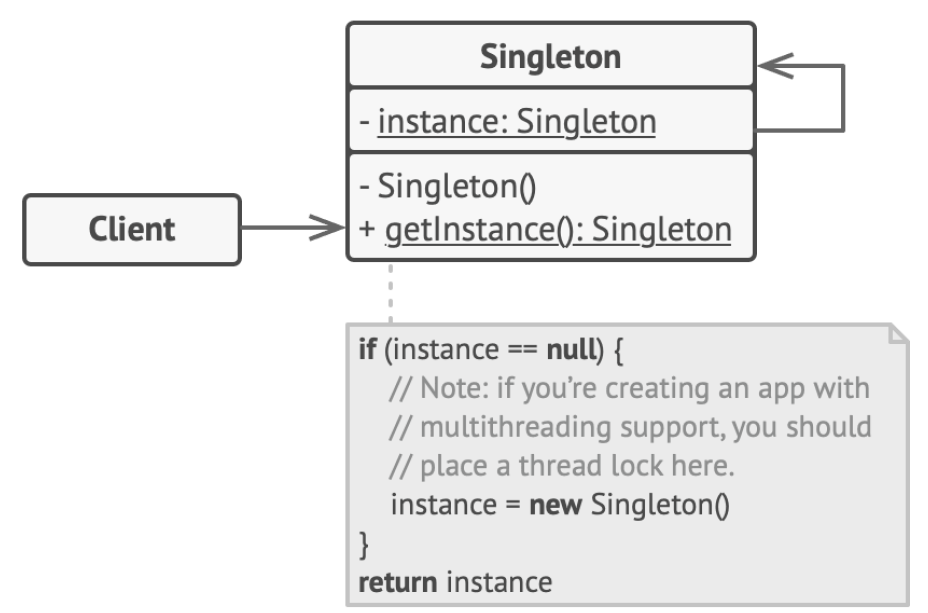
\includegraphics[width=\textwidth]{figures/05.png}
	\caption{功能状态UML图}
	\label{fig:functional_state_diagram}
\end{figure}

初始状态用星号([*])表示,代表用户开始与系统交互。首先,用户访问登录页面,输入账号和密码。在这一阶段,有两个可能的结果:如果验证成功,用户将登录成功并进入服务选择状态;如果验证失败,用户将返回登录页面重新输入账号密码。

在服务选择状态,用户有多个选项,包括查看医生列表、查询处方、访问电子病历、参与医疗服务评价、查看科室信息、预约挂号与问诊服务、时段灵活性与个性化预约、医疗费用账单管理以及缴费与退费流程。每个选项都对应一个动作,用户可以根据自己的需求选择相应的服务。

如果用户选择预约挂号与问诊服务,他们将完成问诊,并接收电子问诊单,随后进入电子问诊单与后续跟进状态。在这里,用户可以查看问诊单详情,并根据需要进行后续操作。

当用户选择时段灵活性与个性化预约,他们将进行预约并确认预约时间。一旦预约成功,状态图将结束,表示用户已经完成了预约流程。

在缴费与退费流程中,用户需要完成在线支付。支付成功后,用户将回到服务选择状态,可以选择其他服务或结束当前会话。

医疗费用账单管理允许用户查看费用账单。用户可以查看详细的费用清单,并在需要时进行支付或其他相关操作。

查询处方和访问电子病历状态允许用户查看处方详情和病历详情,以便更好地了解自己的医疗状况和历史记录。

参与医疗服务评价状态鼓励用户对所接受的服务进行评价,这有助于医疗机构改进服务质量。

最后,每个服务的结束都将用户带回服务选择状态,用户可以选择继续使用其他服务或结束当前会话。当用户结束所有服务时,他们将退出系统,状态图也随之结束。


\subsection{类图}
\subsubsection{用户类图}
用户类图展示了用户账户的基本属性和行为。用户(User)类包含用户名(username)、密码(password)、电子邮件(email)以及与用户相关的处方(Prescriptions)和医疗记录(MedicalRecords)的列表。用户可以进行预约(makeAppointment)、咨询医生(consultDoctor)、查看处方(viewPrescriptions)和查看医疗记录(viewMedicalRecords)。

处方(Prescription)类包含处方ID(prescriptionID)、开具日期(date)、开处方的医生姓名(doctorName)和处方详情(details)。医疗记录(MedicalRecord)类包含记录ID(recordID)、记录日期(date)、医生姓名(doctorName)、诊断(diagnosis)和治疗信息(treatment)。
\begin{figure}[htbp]
	\centering
	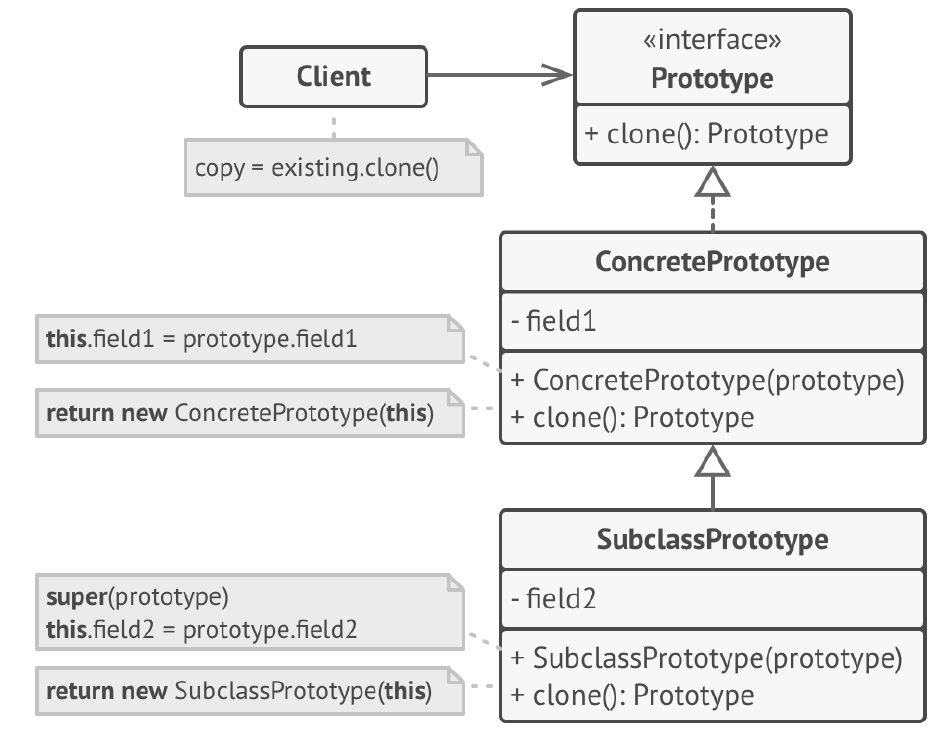
\includegraphics[width=0.4\textwidth]{figures/04.png}
	\caption{功能状态UML图}
	\label{fig:functional_state_diagram}
\end{figure}

\subsubsection{预约与问诊服务类图}
预约与问诊服务类图描述了预约系统的结构和行为。预约服务(AppointmentService)类负责创建(makeAppointment)和取消(cancelAppointment)预约。预约(Appointment)类包含预约时间(datetime)、负责的医生(doctor)、预约的用户(user)和预约状态(status)。状态(Status)枚举定义了预约的可能状态,包括已安排(Scheduled)、已取消(Cancelled)和已完成(Completed)。

医生(Doctor)类包含医生ID(doctorID)、姓名(name)、专业(specialty)和医生的预约列表(appointments)。医生可以进行咨询(consult)。咨询服务(ConsultationService)类提供进行咨询(conductConsultation)、提供处方(providePrescription)和提供医疗记录(provideMedicalRecord)的行为。
\begin{figure}[htbp]
	\centering
	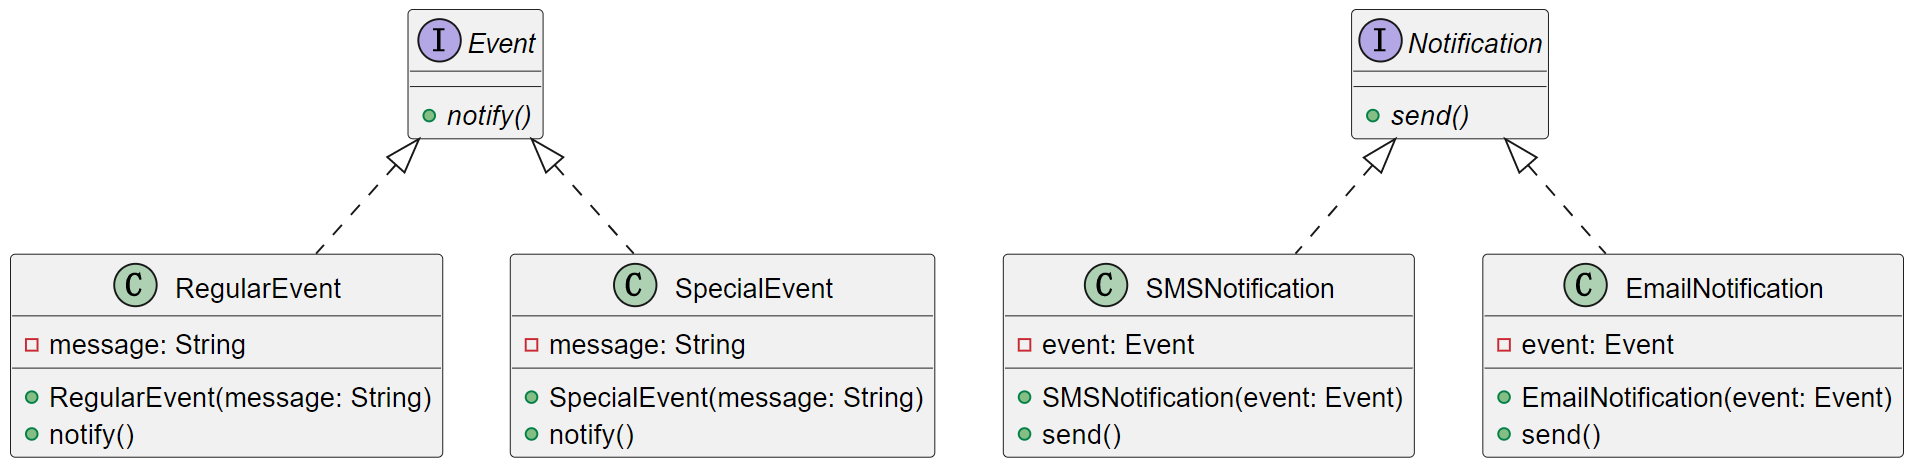
\includegraphics[width=0.76\textwidth]{figures/06.png}
	\caption{功能状态UML图}
	\label{fig:functional_state_diagram}
\end{figure}

\subsubsection{医疗服务评价体系类图}
医疗服务评价体系类图展示了评价系统的结构。评价系统(EvaluationSystem)类负责收集提交的评价(submitEvaluation)和查看医生的评价(viewEvaluations)。评价(Evaluation)类包含评价ID(evaluationID)、评价用户(user)、被评价的医生(doctor)、评价内容(content)、评分(rating)和评价日期(datetime)。

医生(Doctor)类在评价体系中增加了接收评价(receiveEvaluation)的行为。评价(Evaluation)类与用户(User)和医生(Doctor)类相关联,表示评价由用户提交,并且针对特定的医生。

这些类图构成了综合医疗服务系统的基础模型,涵盖了用户交互、预约管理、问诊服务和评价体系等多个方面。通过这些类和它们之间的关系,系统能够管理用户的医疗信息、提供预约和咨询服务,并收集用户对医疗服务的评价。
\begin{figure}[htbp]
	\centering
	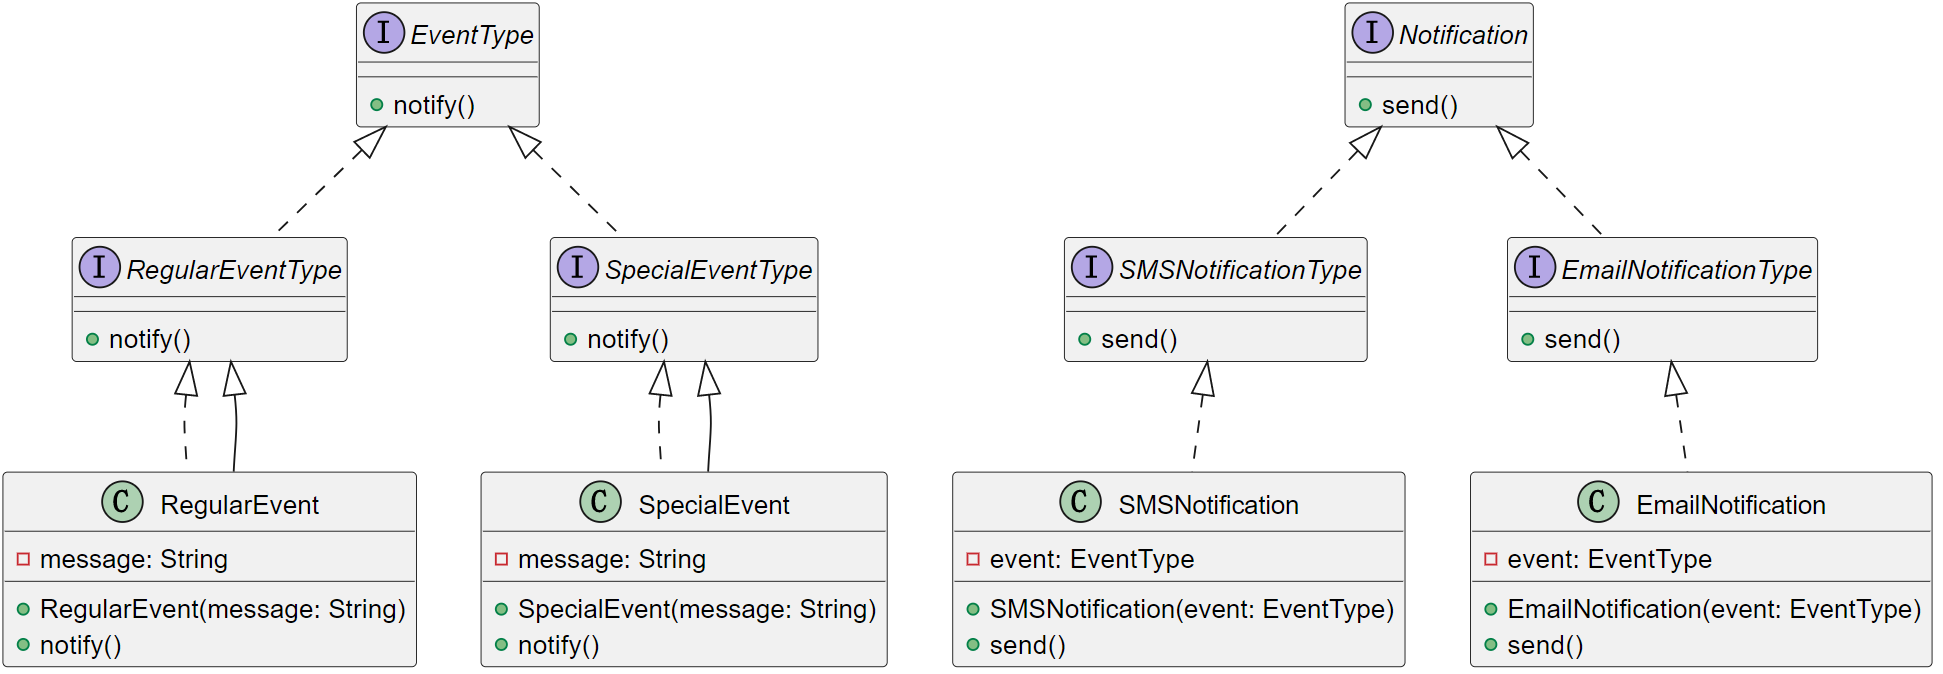
\includegraphics[width=0.6\textwidth]{figures/07.png}
	\caption{功能状态UML图}
	\label{fig:functional_state_diagram}
\end{figure}

\subsubsection{类:普通用户(Ordinary Users)}
\begin{table}[htbp]
	\centering
	\begin{tabular}{|l|l|l|}
		\hline
		\textbf{类} & \textbf{职责} & \textbf{协作者} \\
		\hline
		ordinary users & 用户登录 & User Interface \\
		& 查询举措(measure information) & Measure Database \\
		& 使用论坛(forum) & Forum \\
		& 论坛举报(report forum) & Report System \\
		& 查看医院信息(hospital information) & Hospital Database \\
		& 预约医生(appointment system) & Appointment System \\
		& 使用AI医生问诊(AI doctor) & AI System \\
		& 使用视频通话会诊(video consultation) & Video Conference System \\
		\hline
	\end{tabular}
	\caption{普通用户类的职责和协作者}
	\label{tab:ordinary_users}
\end{table}

普通用户类(ordinary users)代表了使用我们医疗预约管理系统的病人。他们可以通过用户登录功能(user login)访问系统,该功能由用户界面(User Interface)提供支持,并与用户数据库(User Database)协作以验证用户信息。普通用户还可以查询医疗举措信息(measure information),参与论坛讨论(forum),并在必要时进行论坛举报(report forum)。此外,他们可以查看医院信息(hospital information),预约医生(appointment system),使用 AI 医生进行问诊(AI doctor),并通过视频通话进行会诊(video consultation)。

\subsubsection{类:用户登录(User Login)}
\begin{table}[htbp]
	\centering
	\begin{tabular}{|l|l|l|}
		\hline
		\textbf{类} & \textbf{职责} & \textbf{协作者} \\
		\hline
		User Login & 验证用户信息(validate user credentials) & User Database \\
		& 提供登录反馈(provide login feedback) & User Interface \\
		\hline
	\end{tabular}
	\caption{用户登录类的职责和协作者}
	\label{tab:user_login}
\end{table}

用户登录类(User Login)负责处理用户的登录过程。它与用户数据库(User Database)协作以验证用户的凭据,并提供登录反馈给用户界面(User Interface)。

\subsubsection{类:举措信息(Measure Information)}
\begin{table}[htbp]
	\centering
	\begin{tabular}{|l|l|l|}
		\hline
		\textbf{类} & \textbf{职责} & \textbf{协作者} \\
		\hline
		Measure Information & 提供举措信息(provide measure info) & Measure Database \\
		& 提供举措查询(perform measure query) & User Interface \\
		\hline
	\end{tabular}
	\caption{举措信息类的职责和协作者}
	\label{tab:measure_information}
\end{table}

举措信息类(Measure Information)负责向普通用户提供医疗举措的相关信息。它从举措数据库(Measure Database)中获取信息,并通过用户界面(User Interface)提供查询服务。

\subsubsection{类:论坛(Forum)}
\begin{table}[htbp]
	\centering
	\begin{tabular}{|l|l|l|}
		\hline
		\textbf{类} & \textbf{职责} & \textbf{协作者} \\
		\hline
		Forum & 初始化论坛板块(initialize forum boards) & Board Management System \\
		& 管理用户帖子(manage user posts) & Post Management System \\
		& 审核用户评论(moderate user comments) & Comment Moderation Rules \\
		& 提供论坛交流(enable forum interaction) & User Interface \\
		& 处理论坛举报(handle forum reports) & Report System \\
		\hline
	\end{tabular}
	\caption{论坛类的职责和协作者}
	\label{tab:forum}
\end{table}

论坛类(Forum)负责提供一个平台,让用户能够就医疗话题进行交流和讨论。它还负责管理论坛的帖子和用户评论,确保讨论的秩序和内容的适当性。此外,论坛类与用户界面(User Interface)协作,提供论坛交流功能,并与报告系统(Report System)协作,处理用户的举报。

\subsubsection{类:医院信息(Hospital Information)}
\begin{table}[htbp]
	\centering
	\begin{tabular}{|l|l|l|}
		\hline
		\textbf{类} & \textbf{职责} & \textbf{协作者} \\
		\hline
		Hospital Information & 提供医院概况(provide hospital overview) & Hospital Database \\
		& 展示科室信息(display department info) & Department Catalog \\
		& 更新医院新闻(update hospital news) & News System \\
		& 提供医院查询(enable hospital search) & User Interface \\
		\hline
	\end{tabular}
	\caption{医院信息类的职责和协作者}
	\label{tab:hospital_information}
\end{table}

医院信息类(Hospital Information)负责存储和管理与医院相关的所有信息,包括医院概况、科室信息和最新新闻。它通过用户界面(User Interface)提供医院查询功能,使用户能够轻松找到所需的医院信息。

\subsubsection{类:预约系统(Appointment System)}
\begin{table}[htbp]
	\centering
	\begin{tabular}{|l|p{0.5\linewidth}|l|}
		\hline
		\textbf{类} & \textbf{职责} & \textbf{协作者} \\
		\hline
		Appointment System & 检查医生可用性(check doctor availability) & Doctor Schedule \\
		& 安排预约时间(安排预约时间) & Calendar System \\
		& 确认预约(confirm appointments) & User Interface \\
		& 提供预约反馈(provide appointment feedback) & User Interface \\
		& 管理取消和重新预约(manage cancellations and reschedules) & Cancellation Policy \\
		\hline
	\end{tabular}
	\caption{预约系统类的职责和协作者}
	\label{tab:appointment_system}
\end{table}

预约系统类(Appointment System)负责处理用户与医生之间的预约安排。它检查医生的时间表(Doctor Schedule),安排预约时间(Calendar System),并在用户界面(User Interface)上确认预约和提供反馈。此外,它还管理取消和重新预约的流程(Cancellation Policy)。

\subsubsection{类:视频会诊(Video Consultation)}
\begin{table}[htbp]
	\centering
	\begin{tabular}{|l|l|l|}
		\hline
		\textbf{类} & \textbf{职责} & \textbf{协作者} \\
		\hline
		Video Consultation & 初始化视频通话(initialize video calls) & Video Call System \\
		& 管理会诊连接(manage consultation connections) & Network Services \\
		& 录制会诊记录(record consultation records) & Recording System \\
		& 提供会诊反馈(provide consultation feedback) & User Interface \\
		\hline
	\end{tabular}
	\caption{视频会诊类的职责和协作者}
	\label{tab:video_consultation}
\end{table}

视频会诊类(Video Consultation)负责设置和管理在线视频会诊的过程。它使用视频通话系统(Video Call System)来初始化和维护会诊连接,并确保网络服务(Network Services)的稳定性。此外,它还负责录制会诊记录(Recording System),并在会诊结束后通过用户界面(User Interface)提供反馈。

\subsubsection{类:AI医生(AI Doctor)}
\begin{table}[htbp]
	\centering
	\begin{tabular}{|l|l|l|}
		\hline
		\textbf{类} & \textbf{职责} & \textbf{协作者} \\
		\hline
		AI Doctor & 提供医疗咨询(provide medical consultation) & User Interface \\
		& 分析症状(analyze symptoms) & Symptom Analysis Engine \\
		& 推荐治疗方案(recommend treatment plans) & Treatment Database \\
		& 回答健康相关问题(answer health-related questions) & Health Knowledge Base \\
		& 更新患者健康记录(update patient health records) & Patient Record System \\
		\hline
	\end{tabular}
	\caption{AI医生类的职责和协作者}
	\label{tab:ai_doctor}
\end{table}

AI医生类(AI Doctor)通过用户界面(User Interface)提供医疗咨询服务,分析用户输入的症状,并利用症状分析引擎(Symptom Analysis Engine)来识别可能的健康问题。它还可以推荐治疗方案,并从治疗数据库(Treatment Database)中检索相关信息。此外,AI医生类负责回答用户关于健康的问题,并更新患者的健康记录。

\subsubsection{类:视频会诊(Video Consultation)}
\begin{table}[htbp]
	\centering
	\begin{tabular}{|l|p{0.45\linewidth}|l|}
		\hline
		\textbf{类} & \textbf{职责} & \textbf{协作者} \\
		\hline
		Video Consultation & 初始化视频通话(initialize video calls) & Video Call System \\
		& 管理会诊连接(manage consultation connections) & Network Services \\
		& 录制会诊记录(record consultation records) & Recording System \\
		& 提供会诊反馈(provide consultation feedback) & User Interface \\
		& 调度会诊资源(dispatch consultation resources) & Resource Management System \\
		\hline
	\end{tabular}
	\caption{视频会诊类的职责和协作者}
	\label{tab:video_consultation}
\end{table}

视频会诊类(Video Consultation)负责设置和管理在线视频会诊的过程。它使用视频通话系统(Video Call System)来初始化和维护会诊连接,并确保网络服务(Network Services)的稳定性。此外,它还负责录制会诊记录(Recording System),并在会诊结束后通过用户界面(User Interface)提供反馈。视频会诊类还与资源管理系统(Resource Management System)协作,以调度所需的会诊资源。

\subsubsection{类:管理员(Admin)}
\begin{table}[htbp]
	\centering
	\begin{tabular}{|l|l|l|}
		\hline
		\textbf{类} & \textbf{职责} & \textbf{协作者} \\
		\hline
		Admin & 管理用户信息(manage user information) & User Database \\
		& 管理医生信息(manage doctor information) & Doctor Database \\
		& 管理医院信息(manage hospital information) & Hospital Database \\
		& 处理举报信息(handle report information) & Report System \\
		& 监控系统性能(monitor system performance) & Performance Monitoring Tools \\
		& 配置系统设置(configure system settings) & Configuration Manager \\
		\hline
	\end{tabular}
	\caption{管理员类的职责和协作者}
	\label{tab:admin}
\end{table}

管理员类(Admin)负责维护医疗预约管理系统的整体运行。它管理用户数据库(User Database)中的用户信息,包括注册、更新和删除用户账户。管理员还管理医生数据库(Doctor Database)中的医生信息,以及医院数据库(Hospital Database)中的医院信息。此外,管理员处理系统中的举报信息,并监控系统性能,确保系统稳定运行。管理员还可以配置系统设置,以优化系统性能和用户体验。

\subsubsection{类:医生(Doctor)}
\begin{table}[htbp]
	\centering
	\begin{tabular}{|l|p{0.5\linewidth}|l|}
		\hline
		\textbf{类} & \textbf{职责} & \textbf{协作者} \\
		\hline
		Doctor & 提供医疗咨询(provide medical consultation) & User Interface \\
		& 管理预约信息(manage appointment information) & Appointment System \\
		& 参与视频会诊(participate in video consultations) & Video Consultation \\
		& 更新患者处方(update patient prescriptions) & Prescription Management System \\
		& 记录诊断和治疗建议(record diagnoses and treatment suggestions) & Medical Record System \\
		\hline
	\end{tabular}
	\caption{医生类的职责和协作者}
	\label{tab:doctor}
\end{table}

医生类(Doctor)负责向病人提供专业的医疗服务。他们通过用户界面(User Interface)提供医疗咨询,并管理预约系统(Appointment System)中的预约信息。医生还参与视频会诊(Video Consultation),并使用处方管理系统(Prescription Management System)更新患者的处方。此外,医生在医疗记录系统(Medical Record System)中记录诊断和治疗建议,以便跟踪患者的健康状况。
\subsubsection{类:账单管理(Billing Management)}
\begin{table}[htbp]
	\centering
	\begin{tabular}{|l|p{0.5\linewidth}|l|}
		\hline
		\textbf{类} & \textbf{职责} & \textbf{协作者} \\
		\hline
		Billing Management & 生成和发送账单(generate and send bills) & User Interface \\
		& 管理账单支付(manage bill payments) & Payment Gateway \\
		& 处理退款请求(process refund requests) & Financial System \\
		& 提供账单查询和历史记录(provide bill inquiries and history) & Billing Database \\
		\hline
	\end{tabular}
	\caption{账单管理类的职责和协作者}
	\label{tab:billing_management}
\end{table}

账单管理类(Billing Management)负责处理系统中所有与账单相关的事务。它生成和发送账单给用户,管理账单支付过程,并通过支付网关(Payment Gateway)处理用户的支付。此外,它还处理用户的退款请求,并与财务系统(Financial System)协作。账单管理类还提供账单查询和历史记录的功能,让用户能够轻松访问自己的账单信息。

\subsubsection{类:处方管理(Prescription Management)}
\begin{table}[htbp]
	\centering
	\begin{tabular}{|l|p{0.45\linewidth}|l|}
		\hline
		\textbf{类} & \textbf{职责} & \textbf{协作者} \\
		\hline
		Prescription Management & 创建和管理处方(create and manage prescriptions) & Doctor \\
		& 跟踪处方状态(track prescription status) & Pharmacy System \\
		& 提供药物信息(provide drug information) & Drug Database \\
		& 处理处方续签请求(handle prescription renewals) & Medical Record System \\
		\hline
	\end{tabular}
	\caption{处方管理类的职责和协作者}
	\label{tab:prescription_management}
\end{table}

处方管理类(Prescription Management)负责创建和管理医生开具的处方。它跟踪处方的状态,并与药房系统(Pharmacy System)协作,确保药物按时送达。处方管理类还提供药物信息,并处理处方续签请求。它与医疗记录系统(Medical Record System)紧密协作,确保处方信息的准确性和可追溯性。

\subsubsection{类:健康档案管理(Health Record Management)}
\begin{table}[htbp]
	\centering
	\begin{tabular}{|l|p{0.45\linewidth}|l|}
		\hline
		\textbf{类} & \textbf{职责} & \textbf{协作者} \\
		\hline
		Health Record Management & 维护病人健康档案(maintain patient health records) & Doctor \\
		& 更新医疗记录(update medical records) & Billing Management \\
		& 提供健康档案访问(provide health record access) & User Interface \\
		& 保护病人隐私(protect patient privacy) & Security System \\
		\hline
	\end{tabular}
	\caption{健康档案管理类的职责和协作者}
	\label{tab:health_record_management}
\end{table}

健康档案管理类(Health Record Management)负责维护和更新病人的健康档案。它确保医疗记录的准确性和完整性,并在用户界面(User Interface)上提供健康档案的访问。健康档案管理类还保护病人的隐私,并与安全系统(Security System)协作,确保所有健康信息的安全。

\subsubsection{类:报告和分析(Reporting \& Analytics)}
\begin{table}[htbp]
	\centering
	\begin{tabular}{|l|p{0.45\linewidth}|l|}
		\hline
		\textbf{类} & \textbf{职责} & \textbf{协作者} \\
		\hline
		Reporting \& Analytics & 生成医疗报告(generate medical reports) & Health Record Management \\
		& 分析医疗服务使用情况(analyze service usage) & Data Analysis Tools \\
		& 提供决策支持(provide decision support) & Admin \\
		& 监控服务质量(monitor service quality) & Quality Control System \\
		\hline
	\end{tabular}
	\caption{报告和分析类的职责和协作者}
	\label{tab:reporting_analytics}
\end{table}

报告和分析类(Reporting \& Analytics)负责生成医疗报告,并分析医疗服务的使用情况。它为管理员提供决策支持,并监控服务质量。报告和分析类使用数据分析工具(Data Analysis Tools)来处理和解释数据,确保管理层能够基于数据做出明智的决策。

通过添加这些类,我们的病人预约系统将能够提供更加全面和高效的医疗服务,满足病人和医疗服务提供者的各种需求。这些类的职责和协作者之间的关系确保了系统的整体性能和用户体验。

\subsubsection{类:保险处理(Insurance Processing)}
\begin{table}[htbp]
	\centering
	\begin{tabular}{|l|p{0.5\linewidth}|l|}
		\hline
		\textbf{类} & \textbf{职责} & \textbf{协作者} \\
		\hline
		Insurance Processing & 验证保险信息(validate insurance information) & Insurance Company API \\
		& 处理保险索赔(process insurance claims) & Billing Management \\
		& 更新保险状态(update insurance status) & Patient Record System \\
		& 提供保险相关咨询(provide insurance consultation) & User Interface \\
		\hline
	\end{tabular}
	\caption{保险处理类的职责和协作者}
	\label{tab:insurance_processing}
\end{table}

保险处理类(Insurance Processing)负责验证病人的保险信息,并与保险公司的API进行交互以处理索赔。它更新病人的健康档案系统中的保险状态,并提供用户界面上的保险相关咨询服务。

\subsubsection{类:预约提醒(Appointment Reminders)}
\begin{table}[htbp]
	\centering
	\begin{tabular}{|l|p{0.5\linewidth}|l|}
		\hline
		\textbf{类} & \textbf{职责} & \textbf{协作者} \\
		\hline
		Appointment Reminders & 安排预约提醒(schedule appointment reminders) & User Interface \\
		& 发送预约通知(send appointment notifications) & Notification System \\
		& 跟踪提醒状态(track reminder status) & Appointment System \\
		& 管理提醒偏好(manage reminder preferences) & User Profile System \\
		\hline
	\end{tabular}
	\caption{预约提醒类的职责和协作者}
	\label{tab:appointment_reminders}
\end{table}

预约提醒类(Appointment Reminders)负责安排并通过通知系统(Notification System)发送预约提醒,确保病人不会错过他们的预约时间。它还跟踪提醒的状态,并管理用户在用户档案系统(User Profile System)中的提醒偏好设置。

\subsubsection{类:在线支付(Online Payment)}
\begin{table}[htbp]
	\centering
	\begin{tabular}{|l|p{0.5\linewidth}|l|}
		\hline
		\textbf{类} & \textbf{职责} & \textbf{协作者} \\
		\hline
		Online Payment & 处理在线支付事务(process online payments) & Payment Gateway \\
		& 确认支付状态(confirm payment status) & Billing Management \\
		& 提供支付历史记录(provide payment history) & User Interface \\
		& 支持多种支付方式(support multiple payment methods) & Payment Service Providers \\
		\hline
	\end{tabular}
	\caption{在线支付类的职责和协作者}
	\label{tab:online_payment}
\end{table}

在线支付类(Online Payment)负责处理系统中的所有在线支付事务。它与支付网关(Payment Gateway)和支付服务提供商(Payment Service Providers)协作,确认支付状态,并在用户界面(User Interface)上提供支付历史记录。这个类支持多种支付方式,以满足不同用户的需求。

\subsubsection{类:用户反馈(User Feedback)}
\begin{table}[htbp]
	\centering
	\begin{tabular}{|l|p{0.5\linewidth}|l|}
		\hline
		\textbf{类} & \textbf{职责} & \textbf{协作者} \\
		\hline
		User Feedback & 收集用户反馈(collect user feedback) & User Interface \\
		& 分析反馈数据(analyze feedback data) & Reporting \& Analytics \\
		& 响应用户评论(respond to user comments) & Forum \\
		& 改善服务质量(improve service quality) & Service Improvement Team \\
		\hline
	\end{tabular}
	\caption{用户反馈类的职责和协作者}
	\label{tab:user_feedback}
\end{table}

用户反馈类(User Feedback)负责收集和分析用户反馈数据,以便不断改善服务质量。它响应用户在论坛上的评论,并与服务改进团队(Service Improvement Team)协作,根据用户反馈采取行动。

\subsection{数据词典}
\subsubsection{数据流定义表}
\begin{table}[htbp]
	\centering
	\begin{tabular}{|l|p{4cm}|p{4cm}|p{4cm}|}
		\hline
		\textbf{数据流名称} & \textbf{来源/去向} & \textbf{内容} & \textbf{注释} \\
		\hline
		用户登录信息 & 普通用户 
		→ 系统 & 用户名,密码 & 用于验证用户的身份 \\
		预约请求 & 普通用户 
		→ 预约系统 & 用户ID,医生ID,预约时间 & 用于创建新的预约 \\
		预约反馈 & 预约系统 
		→ 普通用户 & 预约状态,预约时间,医生信息 & 用于告知用户预约的结果 \\
		医生信息查询 & 普通用户 
		→ 医生数据库 & 医生ID & 用于获取医生的详细信息 \\
		医生信息 & 医生数据库 
		→ 普通用户 & 医生姓名,专长,可预约时间 & 用于展示医生的详细信息 \\
		举报信息 & 普通用户 
		→ 管理员 & 用户ID,被举报内容,举报理由 & 用于处理用户的举报 \\
		管理操作 & 管理员 
		→ 用户数据库/医生数据库/医院数据库 & 操作类型,目标ID,新信息 & 用于更新数据库的信息 \\
		AI问诊请求 & 普通用户 
		→ AI医生 & 用户ID,病症描述 & 用于AI医生进行诊断 \\
		AI诊断结果 & AI医生 
		→ 普通用户 & 诊断结果,建议的治疗方案 & 用于告知用户AI医生的诊断结果 \\
		视频会诊请求 & 普通用户 
		→ 视频会诊 & 用户ID,医生ID,预约时间 & 用于安排视频会诊 \\
		视频会诊反馈 & 视频会诊 
		→ 普通用户 & 会诊状态,会诊时间,医生信息 & 用于告知用户会诊的结果 \\
		\hline
	\end{tabular}
	\caption{系统中的数据流定义}
	\label{tab:data_flows}
\end{table}
\newpage

\subsubsection{数据元素定义表}
\begin{table}[htbp]
	\centering
	\begin{tabular}{||p{2cm}|l|p{3cm}|p{2cm}|p{2cm}||p{3cm}|}
		\hline
		\textbf{数据元素名称} & \textbf{别名} & \textbf{定义} & \textbf{来源} & \textbf{示例} & \textbf{注释} \\
		\hline
		用户ID & UID & 用户在系统中的唯一标识符 & 用户注册时生成 & 123456 & 用于识别用户 \\
		用户名 & Username & 用户在系统中的名称 & 用户在注册时提供 & JohnDoe & 用于显示用户的名称 \\
		密码 & Password & 用户的登录密码 & 用户在注册时提供 & Password123 & 用于验证用户的身份 \\
		医生ID & DID & 医生在系统中的唯一标识符 & 医生注册时生成 & D78901 & 用于识别医生 \\
		医生姓名 & DoctorName & 医生的姓名 & 医生在注册时提供 & Dr. Smith & 用于显示医生的姓名 \\
		专长 & Specialty & 医生的专长领域 & 医生在注册时提供 & 心脏病专家 & 用于帮助用户选择合适的医生 \\
		可预约时间 & AvailableTime & 医生可接受预约的时间 & 医生提供 & 2024年3月25日 10:00-12:00 & 用于安排预约 \\
		预约时间 & AppointmentTime & 用户预约的时间 & 用户在预约时提供 & 2024年3月25日 11:00 & 用于安排预约 \\
		病症描述 & SymptomDescription & 用户描述的症状信息 & 用户在AI问诊或视频会诊时提供 & 头痛,恶心 & 用于AI医生诊断或医生会诊 \\
		诊断结果 & DiagnosisResult & AI医生或医生的诊断结果 & AI医生或医生提供 & 脑震荡 & 用于告知用户诊断结果 \\
		治疗方案 & TreatmentPlan & AI医生或医生的建议治疗方案 & AI医生或医生提供 & 休息,避免剧烈运动 & 用于指导用户的治疗 \\
		\hline
	\end{tabular}
	\caption{系统中的数据元素定义}
	\label{tab:data_elements}
\end{table}
\newpage

\subsubsection{外部项定义表}

\begin{table}[htbp]
	\centering
	\begin{tabular}{|l|l|l|p{4cm}|p{4cm}|}
		\hline
		\textbf{外部项名称} & \textbf{类型} & \textbf{来源/目的地} & \textbf{内容} & \textbf{注释} \\
		\hline
		用户登录输入 & 输入 & 普通用户 & 用户名,密码 & 用于验证用户的身份 \\
		登录反馈输出 & 输出 & 普通用户 & 用户登录状态,用户信息(如果登录成功) & 用于告知用户登录的结果 \\
		预约请求输入 & 输入 & 普通用户 & 用户ID,医生ID,预约时间 & 用于创建新的预约 \\
		预约反馈输出 & 输出 & 普通用户 & 预约状态,预约时间,医生信息 & 用于告知用户预约的结果 \\
		医生信息查询输入 & 输入 & 普通用户 & 医生ID & 用于获取医生的详细信息 \\
		医生信息反馈输出 & 输出 & 普通用户 & 医生姓名,专长,可预约时间 & 用于展示医生的详细信息 \\
		AI问诊请求输入 & 输入 & 普通用户 & 用户ID,病症描述 & 用于AI医生进行诊断 \\
		AI诊断反馈输出 & 输出 & 普通用户 & 诊断结果,建议的治疗方案 & 用于告知用户AI医生的诊断结果 \\
		视频会诊请求输入 & 输入 & 普通用户 & 用户ID,医生ID,预约时间 & 用于安排视频会诊 \\
		视频会诊反馈输出 & 输出 & 普通用户 & 会诊状态,会诊时间,医生信息 & 用于告知用户会诊的结果 \\
		管理操作输入 & 输入 & 管理员 & 操作类型,目标ID,新信息 & 用于更新数据库的信息 \\
		管理操作反馈输出 & 输出 & 管理员 & 操作结果,新的信息(如果操作成功) & 用于告知管理员操作的结果 \\
		\hline
	\end{tabular}
	\caption{系统中的外部项定义}
	\label{tab:external_entities}
\end{table}
\newpage

\subsubsection{数据精度表}
\begin{table}[htbp]
	\centering
	\begin{tabular}{|l|p{2cm}|p{2cm}|p{2cm}|p{2cm}|p{3cm}|}
		\hline
		\textbf{数据元素名称} & \textbf{数据类型} & \textbf{精度} & \textbf{最小值} & \textbf{最大值} & \textbf{注释} \\
		\hline
		用户ID & 整数 & N/A & 1 & 99999999 & 用户ID应为唯一的正整数 \\
		用户名 & 字符串 & N/A & N/A & 50个字符 & 用户名应不超过50个字符 \\
		密码 & 字符串 & 8个字符 & 20个字符 & N/A & 密码应包含8到20个字符 \\
		医生ID & 整数 & N/A & 1 & 99999999 & 医生ID应为唯一的正整数 \\
		医生姓名 & 字符串 & N/A & N/A & 50个字符 & 医生姓名应不超过50个字符 \\
		专长 & 字符串 & N/A & N/A & 100个字符 & 专长描述应不超过100个字符 \\
		可预约时间 & 日期和时间(分、秒) & 精确到分钟 & 2024年1月1日 00:00 & 2030年12月31日 23:59 & 可预约时间应精确到分钟 \\
		预约时间 & 日期和时间(分、秒) & 精确到分钟 & 2024年1月1日 00:00 & 2030年12月31日 23:59 & 预约时间应精确到分钟 \\
		病症描述 & 字符串 & N/A & N/A & 500个字符 & 病症描述应不超过500个字符 \\
		诊断结果 & 字符串 & N/A & N/A & 500个字符 & 诊断结果应不超过500个字符 \\
		治疗方案 & 字符串 & N/A & N/A & 1000个字符 & 治疗方案应不超过1000个字符 \\
		\hline
	\end{tabular}
	\caption{系统中的数据精度要求}
	\label{tab:data_precision}
\end{table}
\newpage

\subsection{数据流图}
\subsubsection{指令数据流图}
\begin{figure}[htbp]
	\centering
	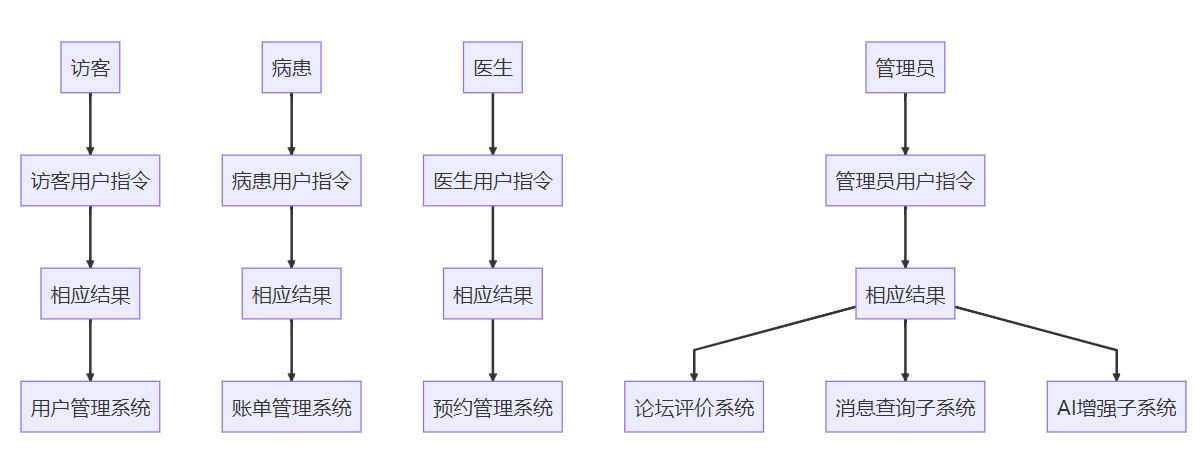
\includegraphics[width=\textwidth]{figures/08.png}
	\caption{指令数据流图}
\end{figure}

\subsubsection{顶层数据流图}
下面是整体的顶层数据流图,由于空间所限,这里放的图较小,更大的可见于附录\ref{app01}。
该顶层数据流图,描述了用户从注册登录到使用各种服务的数据流动过程:
\begin{itemize}
	\item \textbf{用户注册和登录}:用户访问注册页面,填写并提交注册信息。系统验证信息后完成注册,发送确认邮件。用户点击邮件链接激活账户,然后登录系统。
	\item \textbf{个人医疗信息管理}:用户登录后可以查看、更新医疗信息,授权他人访问并查看访问记录,接收系统提示和健康建议。
	\item \textbf{AI医疗咨询服务}:用户提交症状描述,AI系统分析并给出初步建议。用户反馈后,如有需要医生会审核。系统跟踪跟进病情。
	\item \textbf{科室和专业介绍}:用户登录后导航到科室页面,选择并查看感兴趣的科室信息,做出选择。
	\item \textbf{医生预约时间段选择}:用户查看医生列表和可用时间段,选择预约时间段并确认。系统发送确认信息,用户可提交医生评价。
	\item \textbf{医生选择和预约确认}:用户查看医生资料,在线咨询后选择医生。选择就诊时间段,填写预约信息并确认。系统跟踪预约状态。
	\item \textbf{医疗账单管理}:用户提交医疗账单后,可以查看明细。医生或相关人员审核验证后,用户可对项目提出争议。系统发送最终明细,用户在线支付。
	\item \textbf{支付和退款流程}:用户查看未支付费用,选择支付方式完成支付。系统发送确认信息。用户可查看退款政策,申请退款后相关人员审核。系统处理退款并通知用户。
\end{itemize}

\subsubsection{中层数据流图}
下面是整体的中层数据流图,描述了用户从注册登录到使用各种服务的数据流动过程。主要包含下面的内容:
\begin{itemize}
	\item \textbf{用户注册和认证}:用户开始注册,输入并提交注册信息。系统验证信息后,发送确认邮件。用户确认邮件后,注册完成。用户登录时,输入凭证进行验证。验证通过后,用户登录成功。
	\item \textbf{个人健康记录管理}:用户访问健康记录,更新记录并提交。系统验证更新后,更新成功。用户可授权他人访问记录并进行审核。
	\item \textbf{AI辅助咨询}:用户描述症状,AI处理后给出建议。用户与AI交互,如有需要可请求医生审核。
	\item \textbf{预约管理}:用户查看医生可用时间,选择时间段并输入个人信息。提交预约请求后,系统确认时间段,用户可设置提醒和进行就诊后操作。
	\item \textbf{账单和支付管理}:用户查看费用,费用明细后提交支付。系统验证支付后,支付确认。如有差异,用户可提出争议并解决。
	\item \textbf{退款流程}:用户请求退款,管理员审核并处理请求。退款获批后,系统发行退款;否则,退款被拒绝。
\end{itemize}

\subsubsection{病人医生交互}
该交互图\ref{bingren},主要包含下面的内容:
\begin{itemize}
	\item \textbf{病人提交咨询}:病人向医院系统提交咨询。
	\item \textbf{生成病历}:系统根据咨询生成病历。
	\item \textbf{医疗记录}:病历包括过去的测试结果。
	\item \textbf{查询病历}:医生可以查询病历。
	\item \textbf{查看病历}:医生查看病历并进行诊断。
	\item \textbf{诊断结果}:医生给出诊断结果,可能包括开具药方或建议检查。
	\item \textbf{建议检查和药方}:系统将建议检查和药方发送给病人。
	\item \textbf{填写反馈}:病人填写反馈信息。
	\item \textbf{更新病历}:系统更新病历以包括病人的反馈。
	\item \textbf{医院系统}:以上所有交互都发生在医院系统中。
\end{itemize}
\begin{figure}[htbp]
	\centering
	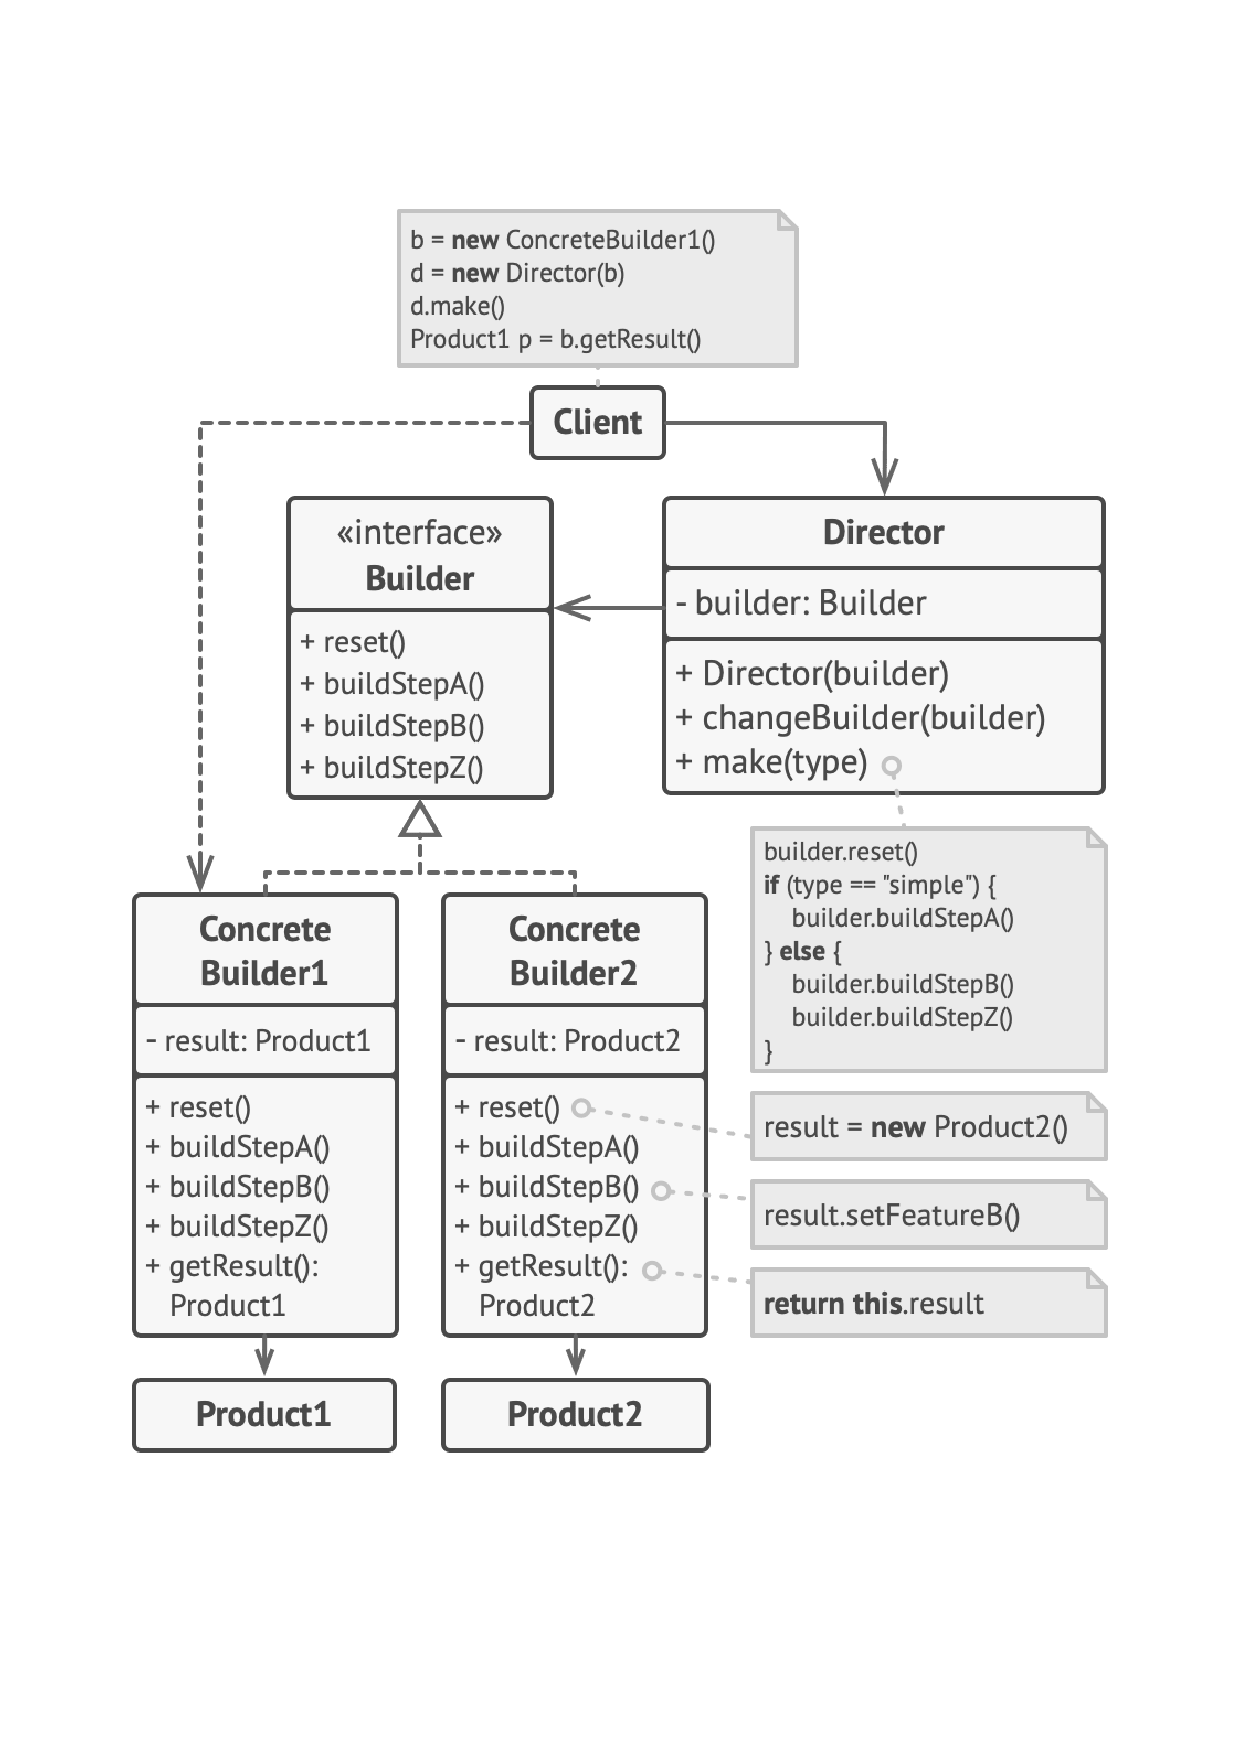
\includegraphics[width=0.9\textwidth]{figures/03.pdf}
	\caption{病人医生交互图}\label{bingren}
\end{figure}